%% Master: ../rough_volterra_lognormal_sv_2026-11-18_btc_eth.tex. Generated by make_qf_version.py: edit the master and regenerate, do not edit this file.
%% Quantitative Finance (rQUF2e) version of rough_volterra_lognormal_sv.tex, derived by
%% make_qf_version.py from the master draft (its revision date is in the master's header). Layout only:
%% no prose or mathematics was changed. The working draft stays the master; regenerate this file after editing it.
%% Location: paper/qf/ (figures are read from ../figures/). Compile: pdflatex -> bibtex -> pdflatex -> pdflatex;
%% rQUF2e.cls and rQUF.bst (from the journal's rquflatex.zip) sit in this folder.
%% Journal rules applied (rQUFguide.tex v2.1): class without options, no geometry package, natbib
%% author-date loaded by the class, \tbl{}{} table captions above the body, figure captions below,
%% no float placement specifiers, references before the appendices, \appendices for the appendix
%% sections, keywords and JEL codes after the abstract, unnumbered Acknowledgements / Disclosure /
%% Supplemental sections before the references.
\RequirePackage[2020-02-02]{latexrelease}% kernel rollback required by rQUF2e v2.1 (2014): kernels from 2020-10 on give
% "Extra \endgroup" at \begin{document}; the 2018-12-01 date in rQUFguide.tex breaks the current graphicx (quoted file names).
% The 2020 kernel rollback requires the matching bundled amsmath release.
\makeatletter\ifdefined\@@eqno\else\let\@@eqno\eqno\fi\makeatother
\RequirePackage{amsmath}[=2018-12-01]
\documentclass{rQUF2e}

\usepackage{booktabs}% compatible with rQUF2e (guide, Section 4.3)
\usepackage{xcolor}% for the \todo markers only; remove with them
\usepackage{url}
\def\UrlBreaks{\do\/\do\_\do\-}
\graphicspath{{../figures/}}% this file lives in paper/qf/, the figures stay in paper/figures/

\theoremstyle{plain}
\newtheorem{theorem}{Theorem}[section]
\newtheorem{proposition}[theorem]{Proposition}
\newtheorem{lemma}[theorem]{Lemma}
\newtheorem{corollary}[theorem]{Corollary}
\newtheorem{conjecture}[theorem]{Conjecture}
\theoremstyle{definition}
\newtheorem{definition}[theorem]{Definition}
\newtheorem{assumption}[theorem]{Assumption}
\theoremstyle{remark}
\newtheorem{remark}[theorem]{Remark}

\newcommand{\D}{\mathrm{d}}
\newcommand{\E}{\mathbb{E}}
\newcommand{\Q}{\mathbb{Q}}
\renewcommand{\P}{\mathbb{P}}
\newcommand{\F}{\mathcal{F}}
\newcommand{\one}{\mathbf{1}}
\newcommand{\VIX}{\mathrm{VIX}}
\newcommand{\todo}[1]{\textcolor{red}{[TODO: #1]}}

\begin{document}



\title{Rough log-normal stochastic volatility with quadratic drift: second-moment stability and the martingale property under positive correlation}

\author{Artur Sepp$^{\ast}$$\dag$\thanks{$^\ast$Corresponding author. Email: \todo{email}} and Parviz Rakhmonov$\ddag$\\
\affil{$\dag$LGT Bank (Schweiz) AG, Z\"urich, Switzerland\\
$\ddag$\todo{Affiliation of Parviz Rakhmonov}}
\received{Working draft, 18 November 2026, Bitcoin and Ether illustrations}}

\maketitle

% [REVISED 2026-10-30 abstract: severity numbers removed (C1), proved content only (C3), xi_0 dropped (C6)]
% [GENERATED 2026-11-17 abstract restated for the results R1-R4]
\begin{abstract}
We extend the log-normal stochastic volatility model with quadratic drift of \citet{SeppRakhmonov2023} to a stochastic Volterra equation with fractional kernel, multiplicative volatility noise and drift $(\kappa_1+\kappa_2\sigma)(\theta-\sigma)$. We prove that the equation has a unique global non-negative strong solution with finite moments for every Hurst exponent $H\in(0,1/2]$. For linear drift we derive exact conditional first and second moments, expected integrated variance and conditional squared VIX. Then the second moment is uniformly bounded in time if and only if $\gamma=\vartheta^2\|G\|_2^2<1$, with $G$ the mean-reversion resolvent and $\gamma$ in closed form, and it grows exponentially for $\gamma>1$. A positive quadratic coefficient $\kappa_2$ removes the restriction in time average. The expected integrated variance per unit time is asymptotically at most $\theta\max(\theta,\kappa_1/\kappa_2)$, for every volatility-of-volatility $\vartheta$ and every $H$. The price is a true martingale when $\kappa_2\ge\beta$, which allows positive spot-volatility correlation. Market prices of risk proportional to volatility preserve the drift polynomial, and the density of the measure change is a true martingale when its quadratic coefficient stays non-negative. A marked order-flow construction explains the drift and noise coefficients, with a stopped diffusion limit for the constant kernel.
\end{abstract}
% [END REVISED 2026-10-30]

% [QF 2026-10-31] keywords and classification codes: journal requirement (three to six keywords, at least one JEL code).
% Suggested by the formatting pass; authors to confirm. MSC 2020 candidates for the cover letter: 60G22, 60H20, 91G20.
\begin{keywords}
Rough volatility; Stochastic Volterra equations; Log-normal stochastic volatility; Quadratic drift; Martingale property; Second-moment stability
\end{keywords}

\begin{classcode}C63; G13\end{classcode}

\section{Introduction}\label{sec:intro}

% [GENERATED 2026-10-08]
Log-volatility of equity indices behaves like a fractional Brownian motion with Hurst exponent of order $0.1$ \citep{GatheralJaissonRosenbaum2018}. \citet{BayerFrizGatheral2016} use this observation in the rough Bergomi model, in which the instantaneous variance is the exponential of a Gaussian Volterra process. The model generates the power-law decay of the at-the-money skew with few parameters. \citet{ElEuchRosenbaum2019} introduce the rough Heston model and derive its characteristic function from a fractional Riccati equation, and \citet{AbiJaberLarssonPulido2019} place it in the class of affine Volterra processes. The quadratic rough Heston model \citep{GatheralJusselinRosenbaum2020} and the quintic Ornstein--Uhlenbeck model \citep{AbiJaberIllandLi2022} extend the class towards joint calibration to SPX and VIX smiles.

% [GENERATED 2026-10-08]
The log-normal stochastic volatility model with quadratic drift of \citet{SeppRakhmonov2023} addresses a different gap. Its volatility follows a diffusion with linear volatility-of-volatility and with drift $(\kappa_1+\kappa_2\sigma)(\theta-\sigma)$. The quadratic term keeps the price process a true martingale when returns and volatility are positively correlated, provided $\kappa_2\ge\beta$, where $\beta$ is the volatility beta. Positive return-volatility correlation is typical for Bitcoin options \citep{SeppRakhmonov2023}. Standard rough Bergomi cannot combine positive spot-volatility correlation with a true-martingale price under the usual pricing measure \citep{Gassiat2019}. In this paper we develop the rough extension of the log-normal model with quadratic drift.

% [AUTHOR PARAGRAPH: economic mechanism]
\todo{Economic mechanism paragraph, drafted by the authors without AI assistance per project rule. Suggested anchor: why volatility shocks should scale with the volatility level and decay as a power law, and why the quadratic drift is the market's response to volatility spikes in assets with positive spot-volatility correlation.}

% [GENERATED 2026-11-17 contributions paragraph restated for the results R1-R4]
We study how quadratic damping interacts with rough memory, multiplicative volatility noise and positive spot-volatility correlation. Theorem~\ref{thm:wellposed} establishes a unique global non-negative strong solution with finite moments for the quadratic drift at every $H\in(0,1/2]$. For linear drift, the conditional first and second moments are exact, and Proposition~\ref{prop:stationarity} characterises uniform long-horizon second-moment boundedness by $\gamma<1$. The threshold has the closed form \eqref{eq:gamma}, and Proposition~\ref{prop:growth} gives the exponential growth rate above it. Since $\vartheta$ has units year$^{-H}$, Table~\ref{tab:critical} also expresses the threshold through a leading-order one-day innovation scale. For quadratic drift, Proposition~\ref{prop:cesaro} bounds the long-run expected integrated variance per unit time by $\theta\max(\theta,\kappa_1/\kappa_2)$, for every $\vartheta$ and every $H$.
% [GENERATED 2026-11-17 final pass] next sentence
The same argument gives the bound \eqref{eq:cesaro_limit_N} for the Markovian kernels used in simulation.
A pointwise long-horizon bound holds for the constant kernel (Proposition~\ref{prop:classical_qd}) and remains open for the fractional kernel. Theorem~\ref{thm:martingale} proves that the price is a true martingale when $\kappa_2\ge\beta$. Proposition~\ref{prop:closure} describes the measure change at the polynomial-coefficient level, and Corollary~\ref{cor:density} gives a sufficient condition for its density to be a true martingale.
% [END GENERATED 2026-11-17]

The expected integrated variance and conditional squared VIX provide exact checks for variance-swap calculations and the inner conditional expectation in VIX pricing (Proposition~\ref{prop:vix}). VIX futures still require an outer expectation of the square root. We compare the split-step Monte Carlo scheme with exact moments of its own Markovian kernel and distinguish sampling error from kernel and time-discretisation error. Appendix~\ref{sec:micro} gives a marked order-flow interpretation and a stopped constant-kernel diffusion limit. The appendix does not establish a global rough microstructural foundation.\footnote{Implementation: \url{https://github.com/ArturSepp/StochVolModels}, module \path{stochvolmodels/pricers/rough_logsv}. Replication scripts are in the folder \path{papers/rough_volterra_lognormal_sv_model_2026/replication} of the same repository.}

% [GENERATED 2026-10-24, revised positioning]
The order-flow interpretation distinguishes the variable moved by a trade from the rate of trading. \citet{HagerHorstWagenhoferXu2026} derive rough Bergomi using i.i.d.\ centred impacts on log-volatility and a constant order rate. \citet{JaissonRosenbaum2016} and \citet{ElEuchFukasawaRosenbaum2018} derive rough Heston from a Hawkes market with one-sided variance impacts. Our proposed construction uses signed volatility impacts and a rate proportional to squared volatility, with a small state-dependent mark bias. The construction is related to the quadratic Hawkes mechanism of \citet{BlancDonierBouchaud2017} and \citet{DandapaniJusselinRosenbaum2021}, but the positive-state and zero-floor identifications require care. Appendix~\ref{sec:micro} separates the exact generator calculation from the open global convergence problem. Section~\ref{sec:model} gives the signed coefficient map to quadratic rough Heston with zero variance floor. With $K\equiv1$, the volatility dynamics reduce to \citet{SeppRakhmonov2023}.

% [REVISED 2026-10-30 positioning against the general martingale criteria (C4)]
The martingale property of prices in Volterra volatility models has a general theory. \citet{Gassiat2019} settles rough Bergomi.
% [GENERATED 2026-11-17 attribution pass] next sentence
\citet{AbiJaberGassiatSotnikov2025} characterise the martingale property when the volatility is a finite linear combination of signature elements of a Brownian motion.
\citet{GuyonJeanninJourdain2026} give general criteria and a localisation reduction to non-explosion under the share measure.
% [GENERATED 2026-11-17 attribution pass] next two sentences
For $\kappa_2=0$ our model belongs to their class. Their results then give a true martingale for $\beta\le0$, and a strict local martingale for $\beta>0$ when the kernel is finite and smooth at zero (Section~\ref{sec:measure}).
In the direct representation of our quadratic drift, their absolute growth restriction in Assumption~1.2 is not satisfied when $\kappa_2>0$, so Theorem~1(B) does not apply directly. Their Lemma~3.1 supplies the localisation principle used in Section~\ref{sec:measure}. We supply the non-explosion step with a one-sided argument. The volatility and the kernel are non-negative, so the quadratic term only lowers the drift (Theorem~\ref{thm:wellposed}).
% [GENERATED 2026-11-17 attribution pass] next sentence
Theorem~\ref{thm:martingale} therefore adds the case $\kappa_2>0$, in which the price is a true martingale under positive correlation when $\kappa_2\ge\beta$.

% [REVISED 2026-10-30 roadmap for the new structure (C5, C7)]
Section~\ref{sec:model} specifies the model, its Markovian approximation, its relation to rough Bergomi and quadratic rough Heston, and its well-posedness. Section~\ref{sec:moments} derives the moments, the stability parameter with its growth rate, and the second-moment bounds under quadratic drift. Section~\ref{sec:measure} proves the martingale property under positive correlation. Section~\ref{sec:illustrations} presents the numerical illustrations. Section~\ref{sec:conclusion} concludes with the open problems. The appendices collect the proofs, the simulation scheme with its validation, the microstructural reading, the notation map and the nearest results.
% [END REVISED 2026-10-30]

\section{Model}\label{sec:model}

\subsection{Dynamics}

% [CARRIED rough_lognormal_sv2.tex Sec. 1, notation aligned with StochVolModels]
We work under the pricing measure $\Q$ with zero interest rates, so that $S_t$ denotes the forward price. The log-normal Volterra stochastic volatility model is
\begin{equation}\label{eq:model}
\begin{split}
\frac{\D S_t}{S_t} &= \sigma_t\,\D W^{(0)}_t,\\
\sigma_t &= \sigma_0+\int_0^t K(t-s)\Big[(\kappa_1+\kappa_2\sigma_s)(\theta-\sigma_s)\,\D s+\beta\sigma_s\,\D W^{(0)}_s+\varepsilon\sigma_s\,\D W^{(1)}_s\Big],
\end{split}
\end{equation}
where $W^{(0)}$ and $W^{(1)}$ are independent Brownian motions. The parameters satisfy $\sigma_0>0$, $\theta>0$, $\kappa_1\ge0$, $\kappa_2\ge0$, $\beta\in\mathbb{R}$ and $\varepsilon>0$. We denote the total volatility-of-volatility and the spot-volatility correlation by
\begin{equation}\label{eq:vartheta}
\vartheta^2=\beta^2+\varepsilon^2,\qquad \rho=\beta/\vartheta,
\end{equation}
and we write $\vartheta\,\D W^{\sigma}_t=\beta\,\D W^{(0)}_t+\varepsilon\,\D W^{(1)}_t$ for the Brownian motion driving the volatility. The kernel is the Riemann--Liouville fractional kernel
\begin{equation}\label{eq:kernel}
K(t)=\frac{t^{H-1/2}}{\Gamma(H+1/2)},\qquad H\in(0,1/2],\qquad \alpha:=H+\tfrac12 .
\end{equation}
For $H=1/2$ the kernel is constant, $K\equiv1$, and \eqref{eq:model} is the model of \citet{SeppRakhmonov2023}. The drift has the polynomial form $(\kappa_1+\kappa_2\sigma)(\theta-\sigma)=\kappa_1\theta-(\kappa_1-\kappa_2\theta)\sigma-\kappa_2\sigma^2$, which we use in the measure changes of Section~\ref{sec:measure}.

% [REVISED 2026-10-30 xi_0 removed from the core model (C6); the multiplier survives in Remark below]
The log-price $X_t=\ln S_t$ and the integrated variance $I_t$ are
\begin{equation}\label{eq:logprice}
X_t=X_0-\frac12 I_t+\int_0^t\sigma_s\,\D W^{(0)}_s,\qquad I_t=\int_0^t\sigma_s^2\,\D s .
\end{equation}

\begin{remark}[Forward variance multiplier]\label{rem:xi}
A bounded, strictly positive deterministic multiplier $\xi_0(t)$ in the price equation, $\D S_t/S_t=\sqrt{\xi_0(t)}\,\sigma_t\,\D W^{(0)}_t$, allows the forward-variance term structure to be fitted without changing the volatility dynamics \eqref{eq:model}. The expected integrated variance is $\int_0^T\xi_0(t)\E[\sigma_t^2]\,\D t$, and a piecewise-constant parameterisation of $\xi_0$ turns calibration to variance-swap maturities into a triangular linear system. The squared-VIX formula carries the same deterministic weight. Under the share measure, the volatility drift gains $\beta\sqrt{\xi_0(t)}\sigma^2$. The analogue of Theorem~\ref{thm:martingale} therefore requires $\kappa_2-\beta\sqrt{\xi_0(t)}\ge0$ for almost every $t\le T$, together with an extension of Theorem~\ref{thm:wellposed} to the time-dependent tilted drift, which we do not prove. For $\beta>0$ the sign condition is $\kappa_2\ge\beta\,\operatorname*{ess\,sup}_{t\le T}\sqrt{\xi_0(t)}$, and for $\beta\le0$ it is automatic. We use $\xi_0\equiv1$ in the main results and implementation.
\end{remark}
% [END REVISED 2026-10-30]

\subsection{Forward volatility curve}

% [CARRIED rough_lognormal_sv2.tex Sec. 3, corrected direction of the kernel]
The volatility \eqref{eq:model} is neither a Markov process nor a semimartingale when $H<1/2$. Following \citet{ViensZhang2019}, we use as state variable the forward volatility curve
\begin{equation}\label{eq:theta_curve}
\Theta^t_s=\sigma_0+\int_0^t K(s-r)\Big[(\kappa_1+\kappa_2\sigma_r)(\theta-\sigma_r)\,\D r+\vartheta\sigma_r\,\D W^\sigma_r\Big],\qquad s\ge t .
\end{equation}
The curve $s\mapsto\Theta^t_s$ is $\F_t$-measurable, satisfies $\Theta^t_t=\sigma_t$, and gives the flow property
\begin{equation}\label{eq:flow}
\sigma_s=\Theta^t_s+\int_t^s K(s-r)\Big[(\kappa_1+\kappa_2\sigma_r)(\theta-\sigma_r)\,\D r+\vartheta\sigma_r\,\D W^\sigma_r\Big],\qquad s\ge t .
\end{equation}
The forward curve is an adapted input to the future Volterra equation and is not in general the conditional mean $\E[\sigma_s\mid\F_t]$. When $t$ advances, the curve moves in the direction $s\mapsto K(s-t)$ on $[t,T]$. This direction enters every functional derivative of the path-dependent Feynman--Kac formula of \citet{ViensZhang2019}. For $K\equiv1$ the curve is flat, $\Theta^t_s=\sigma_t$, and the path-dependent equations reduce to classical partial differential equations.

\subsection{Markovian approximation}

% [CARRIED rough_lognormal_simulation.tex Sec. 1, corrected and aligned with the code]
The implementation replaces $K$ by a sum of exponentials
\begin{equation}\label{eq:kernel_N}
K^N(t)=\sum_{i=1}^N w_i\,e^{-x_i t},\qquad w_i>0,\ x_i\ge0,\qquad \bar w:=\sum_{i=1}^N w_i ,
\end{equation}
with nodes $x_i$ and weights $w_i$ from the quadrature rule of \citet{BayerBreneis2023}, optimised for European options with the longest maturity $T$ of the option chain. Markovian approximations of this type go back to \citet{AbiJaberElEuch2019}, and \citet{AlfonsiKebaier2024} analyse their convergence for completely monotone kernels. The code uses $N=1$ with $x_1=10^{-3}$ and $w_1=1$ for $H\in(0.49,0.5]$, $N=2$ for $H\in(0.4,0.49]$, and $N=3$ for $H\le0.4$. For $H=0.1$ and $T=1$ the rule gives $x=(0.0333,\,2.242,\,46.83)$ and $w=(0.555,\,1.111,\,6.086)$.
% [GENERATED 2026-10-24] next sentence
The rule underestimates the mass of $K^2$, on which the second moment depends, and the implementation offers a fit of the nodes and weights to the moments of the model.\footnote{Module \texttt{kernel\_fit.py} of the package. At $H=0.2$ the fit reduces the largest variance-swap volatility error of the quadrature rule from 255 to 30 basis points (note \texttt{rough\_kernel\_fit\_note.md} in the replication folder).}

\begin{lemma}[Factor representation]\label{lem:factors}
Let $\sigma^N$ solve \eqref{eq:model} with $K^N$ in place of $K$. Define $\sigma_{0,i}=\sigma_0/\bar w$ and let $\sigma^{(i)}$, $i=1,\dots,N$, solve
\begin{equation}\label{eq:factors}
\D\sigma^{(i)}_t=-x_i\big(\sigma^{(i)}_t-\sigma_{0,i}\big)\D t+(\kappa_1+\kappa_2\sigma^N_t)(\theta-\sigma^N_t)\,\D t+\vartheta\sigma^N_t\,\D W^\sigma_t,\qquad \sigma^{(i)}_0=\sigma_{0,i},
\end{equation}
with $\sigma^N_t=\sum_{i=1}^N w_i\sigma^{(i)}_t$. Then $\sigma^N$ solves the Volterra equation with kernel $K^N$, and its forward curve is
\begin{equation}\label{eq:theta_N}
\Theta^{t}_s=\sigma_0+\sum_{i=1}^N w_i\,e^{-x_i(s-t)}\big(\sigma^{(i)}_t-\sigma_{0,i}\big),\qquad s\ge t .
\end{equation}
\end{lemma}

% [GENERATED 2026-10-08]
Lemma~\ref{lem:factors} reduces the approximated model to an $N$-dimensional diffusion, and \eqref{eq:theta_N} expresses the forward curve as a linear function of the factor states. The proof is in Appendix~\ref{app:proofs}. Any choice $\sigma_{0,i}$ with $\sum_i w_i\sigma_{0,i}=\sigma_0$ gives the same $\sigma^N$, and the code uses the equal split $\sigma_{0,i}=\sigma_0/\bar w$.

% [REVISED 2026-10-30 Remark on the one-factor kernel deleted (chronology residue, not load-bearing); text in the 24 October file]

\subsection{Relation to rough Bergomi and quadratic rough Heston}

% [GENERATED 2026-10-08; REVISED 2026-11-17 reduced to one sentence on the constant-kernel case]
Table~\ref{tab:rbergomi} compares the model with rough Bergomi and with quadratic rough Heston. At $H=1/2$ rough Bergomi has Brownian log-volatility, whereas the classical log-normal model with $\kappa_1>0$ and $\kappa_2=0$ has an inverse-gamma invariant law.

\begin{table}
\tbl{Log-normal Volterra model \eqref{eq:model}, rough Bergomi and quadratic rough Heston with zero variance floor.}{%
\begin{tabular}{p{2.5cm}p{3.7cm}p{3.7cm}p{3.7cm}}
\toprule
 & Rough Bergomi & Quadratic rough Heston, $c=0$ & Log-normal Volterra model \\
\midrule
Volatility & $\ln\sigma_t$ Gaussian Volterra process & $\sqrt a\,|Z_t-b|$, where $Z$ solves a Volterra equation with noise $\lambda\eta\sqrt{V_s}\,\D W_s$ & $\sigma_t$ solves a Volterra equation with noise $\vartheta\sigma_s\,\D W^\sigma_s$ \\
Positivity & automatic & non-negative by construction & non-negative (Theorem~\ref{thm:wellposed}); strict positivity open for singular kernels \\
Drift & deterministic log-variance correction and initial curve & linear, level $-\sqrt a\,b$ for the signed state & quadratic, mean reversion to $\theta>0$ \\
Correlation & constant $\rho$ & $\pm1$, sign flips at $Z=b$ & constant $\rho$ \\
Correlation $\rho>0$ & strict local martingale \citep{Gassiat2019} & not studied here & true martingale for $\kappa_2\ge\beta$ (Theorem~\ref{thm:martingale}) \\
Long-horizon second moment & prescribed by the initial forward-variance curve & bounded iff $\gamma<1$ for $b>0$, with $\vartheta=\lambda\eta\sqrt a$ & linear drift, $\kappa_1>0$: bounded iff $\gamma<1$; quadratic drift: time average bounded for every $\vartheta$ (Proposition~\ref{prop:cesaro}) \\
Initial state & deterministic initial forward-variance curve & $Z_0$ through $\theta_0(t)$ & $\sigma_0$ at $t=0$, curve $\Theta^0_s=\sigma_0$ \\
Microstructure & Poisson orders acting on $\ln\sigma$ \citep{HagerHorstWagenhoferXu2026} & related signed quadratic-Hawkes state \citep{DandapaniJusselinRosenbaum2021} & marked order-flow interpretation; global rough limit open \\
\bottomrule
\end{tabular}}
\label{tab:rbergomi}
\end{table}

% [GENERATED 2026-10-24]
Quadratic rough Heston is closer. That model sets $V_t=a(Z_t-b)^2+c$ with $Z_t=\int_0^tK(t-s)\big[\lambda(\theta_0(s)-Z_s)\,\D s+\lambda\eta\sqrt{V_s}\,\D W_s\big]$, and, for $1/2<\alpha<1$, the choice $\theta_0(t)=Z_0t^{-\alpha}/(\lambda\Gamma(1-\alpha))$ of \citet{GatheralJusselinRosenbaum2020} gives $K*(\lambda\theta_0)\equiv Z_0$ for positive times. At $\alpha=1$ we insert $Z_0$ directly as the initial condition instead of using this singular input formula. With $c=0$ the signed volatility $Y_t=\sqrt a\,(Z_t-b)$ solves
\begin{equation}\label{eq:qrh_map}
Y_t=Y_0+\int_0^tK(t-s)\Big[\lambda\big(-\sqrt a\,b-Y_s\big)\,\D s+\lambda\eta\sqrt a\,Y_s\,\D\widetilde W_s\Big],\qquad \D\widetilde W_s=\mathrm{sign}(Y_s)\,\D W_s,
\end{equation}
and the volatility is $|Y|$. Define $\mathrm{sign}(0)=1$, so that $\widetilde W$ has quadratic variation $t$ and is Brownian. The coefficient identification is $\kappa_2=0$, $\kappa_1=\lambda$, $\theta=-\sqrt a\,b$ and $\vartheta=\lambda\eta\sqrt a$. The identification describes a signed equation outside our positive-level, independent-noise parameter class: the transformed Brownian correlation with the price driver is $\mathrm{sign}(Y)$, rather than a fixed $\rho$. Applying absolute value to $Y$ does not commute with the Volterra convolution. Thus this map does not assert that $|Y|$ solves \eqref{eq:model}. Our positive-level specification and the nonlinear drift require their own state-space and well-posedness analysis, which Theorem~\ref{thm:wellposed} provides. For the zero-floor comparison with $b>0$, the signed mean tends to $-\sqrt a\,b\ne0$, which is the condition behind the boundedness entry in Table~\ref{tab:rbergomi}. The proof of Proposition~\ref{prop:stationarity} uses only a non-zero long-run mean, so its criterion applies to the signed state. If $b=0$, that entry need not hold at the critical boundary. For example, at $H=1/2$ the homogeneous equation has a constant second moment when $\vartheta^2=2\lambda$.

\subsection{Well-posedness}

% [GENERATED 2026-11-17 replaces the text of 30 October 2026: global well-posedness for the quadratic drift is proved (R1)]
For $\kappa_2=0$, the drift and diffusion coefficients of \eqref{eq:model} are globally Lipschitz. Theorem~3.3 and Example~2.3(ii) of \citet{AbiJaberLarssonPulido2019} give a unique continuous strong solution for the fractional kernel, and their Lemma~3.1 gives finite-horizon moments. Their Theorem~3.6 and Example~3.7 give a non-negative solution, because the kernel is completely monotone, the boundary drift is $\kappa_1\theta\ge0$, and the diffusion coefficient vanishes at zero. For $\kappa_2>0$ the drift grows quadratically and is not globally Lipschitz, so these results do not apply directly. The next theorem covers the quadratic drift, the tilted drifts of Section~\ref{sec:measure} and the Markovian kernels \eqref{eq:kernel_N}.

\begin{theorem}[Global well-posedness with quadratic drift]\label{thm:wellposed}
Let $K$ be the fractional kernel \eqref{eq:kernel} with $H\in(0,1/2]$ or a Markovian kernel \eqref{eq:kernel_N}. Let $\sigma_0\ge0$, $c_0\ge0$, $c_1\in\mathbb R$, $d\ge0$ and $\vartheta\ge0$, and let $B$ be a Brownian motion. The equation
\begin{equation}\label{eq:sve_general}
\sigma_t=\sigma_0+\int_0^tK(t-s)\big[c_0+c_1\sigma_s-d\sigma_s^2\big]\D s+\int_0^tK(t-s)\vartheta\sigma_s\,\D B_s
\end{equation}
has a pathwise unique continuous strong solution on $[0,\infty)$. The solution is non-negative, and $\E\big[\sup_{t\le T}\sigma_t^p\big]<\infty$ for every $p\ge1$ and $T>0$.
\end{theorem}

The volatility equation in \eqref{eq:model} is \eqref{eq:sve_general} with $c_0=\kappa_1\theta$, $c_1=\kappa_2\theta-\kappa_1$ and $d=\kappa_2$. The proof is in Appendix~\ref{app:proofs}. The difficulty is that a stochastic Volterra equation has no It\^o formula for functions of the state, so the Lyapunov argument that controls a quadratic drift for a diffusion is not available. We replace it by a one-sided bound. A truncated equation has a non-negative solution by the results cited above. On the non-negative half-line the term $-d\sigma^2$ only lowers the drift, and the non-negative kernel carries this sign through the convolution. The moments of the truncated solutions are therefore bounded by those of a linear majorant, uniformly in the truncation level, and we remove the truncation.
% [GENERATED 2026-11-17 attribution pass] next sentence
\citet{PannierJacquier2019} remove a truncation in the same way for a locally Lipschitz drift, under a linear growth condition that excludes the quadratic term.

The moment bound of Theorem~\ref{thm:wellposed} holds on finite horizons and inherits the growth of the linear majorant. Section~\ref{sec:moments} quantifies the long-horizon behaviour. At $H=1/2$ the equation is the classical positive, non-explosive diffusion of \citet{SeppRakhmonov2023}. For $H<1/2$ the theorem gives $\sigma_t\ge0$ and leaves strict positivity open.

\begin{conjecture}[Strict positivity]\label{conj:wellposed}
For every $H\in(0,1/2)$ and the parameters of \eqref{eq:model}, the volatility is almost surely strictly positive on every finite time interval.
\end{conjecture}

No result of this paper uses Conjecture~\ref{conj:wellposed}. Neither zero-hitting paths of a numerical scheme nor the microscopic sign bias of Appendix~\ref{sec:micro_model} resolves it.
% [END GENERATED 2026-11-17]

\section{Moments and the stability parameter}\label{sec:moments}

% [GENERATED 2026-10-08; REVISED 2026-10-30 section title]
With $\kappa_2=0$ the drift is linear, and the volatility solves a linear stochastic Volterra equation with multiplicative noise. The first two conditional moments are then available in closed form up to the resolvent of the kernel. The economic content is simple. Mean reversion acts on the volatility through the kernel, and its cumulative effect is the resolvent. The noise acts through the same kernel filtered by the resolvent, and its second moment compounds through the singularity of the kernel at zero.

\subsection{Resolvent}

Let $R$ denote the resolvent of $\kappa_1K$ \citep[Chapter~2]{GripenbergLondenStaffans1990}, defined by
\begin{equation}\label{eq:resolvent}
R=\kappa_1K-\kappa_1K*R,\qquad (K*R)(t)=\int_0^tK(t-u)R(u)\,\D u,
\end{equation}
and define $G=R/\kappa_1$ for $\kappa_1>0$ and $G=K$ for $\kappa_1=0$. For the fractional kernel \eqref{eq:kernel} the resolvent is explicit \citep{ElEuchRosenbaum2019},
\begin{equation}\label{eq:resolvent_frac}
R(t)=\kappa_1t^{\alpha-1}E_{\alpha,\alpha}(-\kappa_1t^{\alpha}),\qquad \int_0^tR(u)\,\D u=1-E_\alpha(-\kappa_1t^\alpha),\qquad G(t)=t^{\alpha-1}E_{\alpha,\alpha}(-\kappa_1t^{\alpha}),
\end{equation}
where $E_{a,b}(z)=\sum_{k\ge0}z^k/\Gamma(ak+b)$ is the Mittag-Leffler function and $E_a=E_{a,1}$. For the Markovian kernel \eqref{eq:kernel_N} the resolvent follows from a linear system of $N$ ordinary differential equations.

\subsection{Conditional mean and second moment}

\begin{proposition}[Conditional mean]\label{prop:mean}
Let $\kappa_2=0$ and $t\le s$. The conditional mean $m_t(s)=\E[\sigma_s\mid\F_t]$ is
\begin{equation}\label{eq:cond_mean}
m_t(s)=\theta+\psi_t(s)-\int_t^sR(s-r)\,\psi_t(r)\,\D r,\qquad \psi_t(s)=\Theta^t_s-\theta .
\end{equation}
In particular, $m(t):=\E[\sigma_t]=\theta+(\sigma_0-\theta)\big(1-\int_0^tR(u)\,\D u\big)$, and for the fractional kernel $m(t)=\theta+(\sigma_0-\theta)E_\alpha(-\kappa_1t^\alpha)$.
\end{proposition}

\begin{proposition}[Conditional second moment]\label{prop:second}
Let $\kappa_2=0$ and $t\le s$. The conditional second moment $v_t(s)=\E[\sigma_s^2\mid\F_t]$ solves the linear Volterra equation
\begin{equation}\label{eq:cond_second}
v_t(s)=m_t(s)^2+\vartheta^2\int_t^sG(s-r)^2\,v_t(r)\,\D r .
\end{equation}
Equivalently, $v_t=m_t^2+\widetilde R*m_t^2$ on $[t,\infty)$, where $\widetilde R$ is the resolvent of $\vartheta^2G^2$ with positive sign, $\widetilde R=\vartheta^2G^2+\vartheta^2G^2*\widetilde R$.
\end{proposition}

% [GENERATED 2026-10-08]
The proofs are in Appendix~\ref{app:proofs}. The key step writes the centred volatility $\sigma_s-m_t(s)$ as the stochastic convolution $\int_t^sG(s-r)\vartheta\sigma_r\,\D W^\sigma_r$. The deterministic mean reversion is absorbed in the resolvent, and It\^o's isometry then closes the second moment. The cross-time covariances of the volatility never enter \eqref{eq:cond_second}, which is why the equation is linear and one-dimensional.
% [GENERATED 2026-11-17 attribution pass] next three sentences
With $\kappa_2=0$ the drift is affine and the squared diffusion coefficient is quadratic in the state. The volatility is then a polynomial Volterra process in the sense of \citet{AbiJaberCuchieroPelizzariPulidoSvalutoFerro2024}, whose moments solve deterministic integral equations. Propositions~\ref{prop:mean} and~\ref{prop:second} give the first two of these equations in resolvent form.

\begin{corollary}[Mittag-Leffler growth]\label{cor:ml}
Let $\kappa_1=\kappa_2=0$ and let $K$ be the fractional kernel \eqref{eq:kernel}. Then
\begin{equation}\label{eq:ml_second}
\E[\sigma_t^2]=\sigma_0^2\,E_{2H}\big(a\,t^{2H}\big),\qquad a=\frac{\vartheta^2\,\Gamma(2H)}{\Gamma(H+1/2)^2},
\end{equation}
and $\E[I_T]=\sigma_0^2\,T\,E_{2H,2}\big(a\,T^{2H}\big)$. As $t\to\infty$, $\E[\sigma_t^2]\sim(2H)^{-1}\sigma_0^2\exp\big(a^{1/(2H)}t\big)$.
\end{corollary}

% [GENERATED 2026-10-08; REVISED 2026-10-30 units caveat added (C1), chronology removed, Table 2 entry corrected (C2)]
At $H=1/2$ the corollary gives $\E[\sigma_t^2]=\sigma_0^2e^{\vartheta^2t}$, the second moment of a geometric Brownian motion. For $H<1/2$ the rate $a^{1/(2H)}$ can be large, as Table~\ref{tab:growth} illustrates. Across rows, $\vartheta$ is fixed numerically in the different units year$^{-H}$, so the rows do not represent the same market volatility-of-volatility. For the illustrative choice $H=0.2$ and $\vartheta=1.85$, the one-year ratio without mean reversion is $1.3\times10^{19}$. With $\kappa_1=3$ the refined-grid estimate is about $4.8\times10^7$. At $H=0.3$ the ratio falls from $1.5\times10^4$ to $6.2$. In rough Bergomi the second moment of volatility is fixed by the forward variance curve, while higher moments include factors of the form $\exp(c\,t^{2H})$.

\begin{table}
\tbl{One-year ratio $\E[\sigma_1^2]/\sigma_0^2$ with $\sigma_0=\theta$, $\vartheta$ in year$^{-H}$ and $\kappa_1$ in year$^{-(H+1/2)}$. The upper panel evaluates the Mittag-Leffler series of Corollary~\ref{cor:ml} in the log domain, and its largest entry has $\log_{10}$ ratio $7753.46$. The lower panel solves \eqref{eq:cond_second} by product integration on grids of 2000, 4000 and 8000 steps. The entry for $H=0.2$ and $\vartheta=1.85$ changes by $0.054\%$ between 32{,}000 and 64{,}000 steps. The entry for $H=0.1$ and $\vartheta=1.85$ uses the growth rate of Proposition~\ref{prop:growth} and has $\log_{10}$ ratio $7485.72$.}{%
\begin{tabular}{lrrrrrr}
\toprule
 & \multicolumn{3}{c}{$\kappa_1=0$} & \multicolumn{3}{c}{$\kappa_1=3$} \\
\cmidrule(lr){2-4}\cmidrule(lr){5-7}
$H$ & $\vartheta=0.5$ & $\vartheta=1.0$ & $\vartheta=1.85$ & $\vartheta=0.5$ & $\vartheta=1.0$ & $\vartheta=1.85$ \\
\midrule
0.5 & 1.284 & 2.718 & 30.65 & 1.043 & 1.199 & 2.227 \\
0.3 & 1.390 & 5.102 & $1.48\times10^{4}$ & 1.067 & 1.336 & 6.219 \\
0.2 & 1.530 & 17.74 & $1.29\times10^{19}$ & 1.110 & 1.661 & $\approx4.8\times10^{7}$ \\
0.1 & 2.167 & $1.62\times10^{17}$ & $10^{7753}$ & 1.320 & 29.2 & $10^{7486}$ \\
\bottomrule
\end{tabular}}
\label{tab:growth}
\end{table}

% [GENERATED 2026-10-08; REVISED 2026-10-30 implications paragraph, xi_0 reference removed (C6)]
The growth result changes how the model is calibrated. A volatility-of-volatility estimated in the classical model at $H=1/2$ cannot be carried over to $H=0.1$, because the two parameters have different units and the same number produces moments that differ by many orders of magnitude. Monte Carlo estimates of the expected integrated variance become unreliable in the explosive region, since the sample mean of a heavy-tailed variable converges slowly.
% [GENERATED 2026-11-17 final pass] next sentence. Number: ../replication/results/F4_right_panel_time_averaged.json.
Section~\ref{sec:illustrations} gives an example in which 200{,}000 paths understate the exact five-year expected integrated variance by a factor of about $290$.
Calibration should therefore constrain the triple $(H,\vartheta,\kappa_1)$ jointly, and Proposition~\ref{prop:stationarity} below gives the constraint in closed form. We believe the quadratic drift $\kappa_2$ is the natural stabiliser. The quadratic drift removes the constraint for the constant kernel (Proposition~\ref{prop:classical_qd}), and for the fractional kernel it bounds the time-averaged second moment for every $\vartheta$ (Proposition~\ref{prop:cesaro}). The moments for $\kappa_2>0$ and $H<1/2$ are finite on finite horizons by Theorem~\ref{thm:wellposed}, although they are not available in closed form.

\subsection{Long-horizon second-moment stability}\label{sec:stability}

% [GENERATED 2026-10-24; REVISED 2026-10-30 renamed (stability, not stationarity), crux sentence added, exponent corrected, severity restated through the daily innovation (C1). Numbers: ../replication/rough_logsv_stationarity_check.py.]
The growth of Table~\ref{tab:growth} has a threshold. Equation \eqref{eq:cond_second} is a linear Volterra equation with the non-negative kernel $h=\vartheta^2G^2$. Its positive resolvent is $\widetilde R=\sum_{j\ge1}h^{*j}$, and Tonelli's theorem gives $\int_0^\infty\widetilde R=\sum_{j\ge1}\gamma^j$, where $\gamma=\int_0^\infty h$. The series is finite exactly when $\gamma<1$. Since the squared mean is bounded above and away from zero under the next proposition's hypotheses, the same threshold characterises uniform second-moment boundedness.

\begin{proposition}[Long-horizon second-moment stability]\label{prop:stationarity}
Let $\kappa_2=0$, $\kappa_1>0$, $\theta>0$ and $\sigma_0>0$, and define
\begin{equation}\label{eq:gamma}
\begin{split}
\gamma&:=\vartheta^2\int_0^\infty G(u)^2\,\D u,\\
\int_0^\infty G(u)^2\,\D u&=\frac1\pi\int_0^\infty\frac{\D\omega}{\omega^{2\alpha}+2\kappa_1\cos(\pi\alpha/2)\,\omega^\alpha+\kappa_1^2}=C(\alpha)\,\kappa_1^{-2H/(H+1/2)},
\end{split}
\end{equation}
where
\begin{equation*}
C(\alpha)=-\frac{\cot(\pi\alpha/2)}{\alpha\sin(\pi/\alpha)},\qquad \tfrac12<\alpha<1,\qquad C(1)=\tfrac12.
\end{equation*}
Then $\sup_{t\ge0}\E[\sigma_t^2]<\infty$ if and only if $\gamma<1$. If $\gamma<1$, then $\E[\sigma_t^2]\to\theta^2/(1-\gamma)$ as $t\to\infty$, and if $\gamma\ge1$, then $\E[\sigma_t^2]\to\infty$.
\end{proposition}

The proof is in Appendix~\ref{app:proofs}. At $H=1/2$ the condition reads $\vartheta^2<2\kappa_1$, and the limit $2\kappa_1\theta^2/(2\kappa_1-\vartheta^2)$ is the second moment of the inverse gamma stationary law of \citet{SeppRakhmonov2023}. For $\kappa_1=0$ the integral in \eqref{eq:gamma} diverges, which is consistent with Corollary~\ref{cor:ml}. We call $\gamma$ the linear-drift stability parameter. The parameter is also the squared feedback-kernel norm in the signed quadratic-Hawkes comparison in Appendix~\ref{sec:micro}. The criterion concerns the coefficients under the specified measure, and it does not extend unchanged to quadratic drift. In the lower panel of Table~\ref{tab:growth}, the entry $H=0.2$, $\vartheta=1.85$ has $\gamma=1.36$. At $H=0.1$, $\vartheta=1$ the parameter is $\gamma=0.97$ and the long-run limit is $32.8$, of which the one-year value $29.2$ is already $89\%$. The moderate set $(\kappa_1,\vartheta)=(2,0.72)$ has $\gamma=0.58$, $0.26$ and $0.18$ at $H=0.1$, $0.2$ and $0.3$.

% [GENERATED 2026-11-17 attribution pass] paragraph
\citet{Pages2024} and \citet{GnabeyeuPages2025} study Volterra equations with affine drift and a diffusion coefficient whose square is a quadratic polynomial of the state. The linear-drift case of \eqref{eq:model} has this form. These authors multiply the diffusion coefficient by a deterministic function of time, chosen so that the mean and the variance can stay constant. Under a smallness condition, they bound the second moment of the stabilised equation uniformly in time. Proposition~\ref{prop:stationarity} treats the equation without the stabilising function. The proposition gives the condition in both directions and the constant $C(\alpha)$ in closed form, and Proposition~\ref{prop:growth} below adds the growth rate above the threshold.
% [END GENERATED 2026-11-17]

% [GENERATED 2026-11-17 growth rate above the threshold (R4). Numbers: ../replication/rough_logsv_growth_rate.py.]
Above the threshold the second moment grows exponentially, and its rate solves a scalar equation. Define the Laplace transform of the kernel $h=\vartheta^2G^2$,
\begin{equation}\label{eq:h_hat}
\widehat h(\lambda)=\vartheta^2\int_0^\infty e^{-\lambda u}G(u)^2\,\D u
=\frac{\vartheta^2}{\pi}\int_0^\infty\frac{\D\omega}{\big|(\lambda/2+\mathrm{i}\omega)^\alpha+\kappa_1\big|^2},\qquad\lambda>0 .
\end{equation}
The function $\widehat h$ is continuous and strictly decreasing, with $\widehat h(0+)=\gamma$ and $\widehat h(\lambda)\to0$ as $\lambda\to\infty$.

\begin{proposition}[Growth rate above the threshold]\label{prop:growth}
Let $\kappa_2=0$, $\kappa_1\ge0$, $\theta>0$ and $\sigma_0>0$, and set $\gamma=\infty$ when $\kappa_1=0$. If $\gamma>1$, the equation $\widehat h(\lambda^*)=1$ has a unique root $\lambda^*>0$, and
\begin{equation}\label{eq:growth}
\lim_{t\to\infty}e^{-\lambda^*t}\,\E[\sigma_t^2]=\frac{1}{|\widehat h'(\lambda^*)|}\int_0^\infty e^{-\lambda^*s}m(s)^2\,\D s .
\end{equation}
For $\sigma_0=\theta$ the limit equals $\theta^2/(\lambda^*|\widehat h'(\lambda^*)|)$. If $\gamma=1$, then $\E[\sigma_t^2]/t\to\theta^2/\mu_h$ as $t\to\infty$, where $\mu_h=\vartheta^2\int_0^\infty u\,G(u)^2\,\D u<\infty$.
\end{proposition}

The proof in Appendix~\ref{app:proofs} reads \eqref{eq:cond_second} as a renewal equation. For $\kappa_1=0$ the transform is $\widehat h(\lambda)=a\lambda^{-2H}$, so that $\lambda^*=a^{1/(2H)}$ and the limit is $\sigma_0^2/(2H)$, in agreement with Corollary~\ref{cor:ml}. At $H=1/2$ the root is $\lambda^*=\vartheta^2-2\kappa_1$. Mean reversion lowers the rate only moderately when the kernel is rough. At $H=0.1$ and $\vartheta=1.85$ the rate is $17{,}851$ per year for $\kappa_1=0$ and $17{,}235$ per year for $\kappa_1=3$, which gives the last entry of Table~\ref{tab:growth}. The formula agrees with product integration where both are available. For $\gamma=1.2$, $\kappa_1=2$ and $\sigma_0=\theta$, the formula and product integration give $\E[\sigma_5^2]/\theta^2=1.33497\times10^{43}$ and $1.33501\times10^{43}$ at $H=0.1$, and $74{,}174.81$ and $74{,}174.78$ at $H=0.3$.\footnote{These values add the constant $-1/(\gamma-1)$ to the leading term $e^{\lambda^*t}/(\lambda^*|\widehat h'(\lambda^*)|)$. The constant is the formal contribution of the singularity at zero of the Laplace transform of $\E[\sigma_t^2]$, and it is exact at $H=1/2$.}
% [END GENERATED 2026-11-17]

Table~\ref{tab:critical} lists the critical volatility-of-volatility $\vartheta_c=(\int_0^\infty G^2)^{-1/2}$. The second moment is unbounded at and above this threshold. Mean reversion raises it as $\vartheta_c\propto\kappa_1^{H/\alpha}$, with exponent $1/6$ at $H=0.1$ and $1/2$ at $H=1/2$. A tenfold increase of $\kappa_1$ therefore raises $\vartheta_c$ by $47\%$ and $216\%$, respectively. Parameters have Hurst-dependent units, so comparisons across rows require a horizon and a quotation convention. Freezing the volatility coefficient over a short horizon $\Delta$ gives the leading-order innovation proxy
\begin{equation*}
\nu_\Delta=\vartheta\Big(\int_0^\Delta K(u)^2\,\D u\Big)^{1/2}
=\frac{\vartheta\Delta^H}{\sqrt{2H}\,\Gamma(\alpha)}.
\end{equation*}
The proxy reduces to $\vartheta\sqrt\Delta$ at $H=1/2$. The right block of Table~\ref{tab:critical} expresses the boundary using $\nu_{1/252,c}$. The proxy is a short-horizon, frozen-coefficient quantity and not an exact conditional daily standard deviation. The distinction matters especially when the value exceeds one. Whether the linear-drift constraint binds in a market depends on the calibrated triple $(H,\kappa_1,\vartheta)$ with its stated units.

% [GENERATED 2026-11-17 terminology bridge to rough Bergomi units. Numbers: ../replication/rough_logsv_growth_rate.py.]
The proxy also links $\vartheta$ to the volatility-of-volatility $\eta_{\mathrm{B}}$ of rough Bergomi, in which the variance is $\xi_0(t)\,\mathcal{E}\big(\eta_{\mathrm{B}}\sqrt{2H}\int_0^t(t-s)^{H-1/2}\,\D W_s\big)$ \citep{BayerFrizGatheral2016}. Matching the short-time kernels of the log-volatility in the two models gives $\vartheta=\eta_{\mathrm{B}}\sqrt{2H}\,\Gamma(\alpha)/2$ and therefore $\nu_\Delta=(\eta_{\mathrm{B}}/2)\Delta^H$. In these units the critical values of Table~\ref{tab:critical} at $H=0.1$ are $\eta_{\mathrm{B},c}=2.54$, $3.05$ and $3.73$ for $\kappa_1=1$, $3$ and $10$.
% [END GENERATED 2026-11-17]

\begin{table}
\tbl{Critical volatility-of-volatility $\vartheta_c$ in year$^{-H}$ (left block) and the corresponding one-day innovation proxy $\nu_{1/252,c}$ (right block), with $\kappa_1$ in year$^{-(H+1/2)}$. For linear drift, the second moment is uniformly bounded in time exactly when $\vartheta<\vartheta_c$. The proxy is defined by freezing the volatility coefficient over one day. The closed constant was checked against independent spectral quadrature.}{%
\begin{tabular}{lrrrrrrrrrrr}
\toprule
 & & \multicolumn{5}{c}{$\vartheta_c$} & \multicolumn{5}{c}{$\nu_{1/252,c}$} \\
\cmidrule(lr){3-7}\cmidrule(lr){8-12}
$H$ & $C(\alpha)$ & $\kappa_1=1$ & $2$ & $3$ & $5$ & $10$ & $\kappa_1=1$ & $2$ & $3$ & $5$ & $10$ \\
\midrule
0.5 & 0.500 & 1.414 & 2.000 & 2.449 & 3.162 & 4.472 & 0.089 & 0.126 & 0.154 & 0.199 & 0.282 \\
0.4 & 0.515 & 1.394 & 1.897 & 2.272 & 2.851 & 3.879 & 0.160 & 0.217 & 0.260 & 0.327 & 0.444 \\
0.3 & 0.574 & 1.319 & 1.711 & 1.992 & 2.413 & 3.129 & 0.279 & 0.361 & 0.421 & 0.509 & 0.660 \\
0.2 & 0.747 & 1.157 & 1.411 & 1.584 & 1.833 & 2.234 & 0.466 & 0.569 & 0.639 & 0.739 & 0.901 \\
0.1 & 1.398 & 0.846 & 0.949 & 1.016 & 1.106 & 1.241 & 0.730 & 0.820 & 0.877 & 0.955 & 1.072 \\
\bottomrule
\end{tabular}}
\label{tab:critical}
\end{table}
% [END GENERATED 2026-10-24 / REVISED 2026-10-30]

\subsection{Second moment under the quadratic drift}\label{sec:classical_qd}

% [REVISED 2026-10-30 new subsection (C3, C7): the stationary density moved here from the microstructure section, where it was part of the scaling-limit proposition]
The quadratic drift removes the linear-drift second-moment constraint when the kernel is constant. In the generator applied to $\sigma^2$, its contribution is $-2\kappa_2\sigma^3$, which dominates the quadratic diffusion contribution $\vartheta^2\sigma^2$ at large volatility for every $\vartheta$.

\begin{proposition}[Quadratic drift at $H=1/2$]\label{prop:classical_qd}
Let $K\equiv1$, $\kappa_1>0$, $\theta>0$ and $\kappa_2>0$. The stationary density of $\sigma$ is proportional to
\begin{equation}\label{eq:stationary_density}
\sigma^{-2-2(\kappa_1-\kappa_2\theta)/\vartheta^2}\exp\Big(-\frac{2\kappa_1\theta}{\vartheta^2\sigma}-\frac{2\kappa_2\sigma}{\vartheta^2}\Big),
\end{equation}
and every positive and negative moment under the stationary law is finite for every $\vartheta>0$. From any deterministic $\sigma_0>0$, the second moment is uniformly bounded on $[0,\infty)$.
\end{proposition}

The proof is in Appendix~\ref{app:proofs}.
% [GENERATED 2026-11-17 attribution pass] next sentence
The density \eqref{eq:stationary_density} is of generalised inverse Gaussian type, the steady-state law that \citet{CarrWillems2019} obtain for a log-normal volatility with quadratic drift.
With $\kappa_2=0$, \eqref{eq:stationary_density} reduces to the inverse gamma law of \citet{SeppRakhmonov2023}, whose second moment is finite exactly when $\vartheta^2<2\kappa_1$, or $\gamma<1$ at $H=1/2$. With $\kappa_2>0$, the exponential tail gives all stationary moments, and the Lyapunov estimate in the proof gives a uniform second-moment bound from a deterministic initial state.

% [GENERATED 2026-11-17 time-averaged bound (R3), extended to the kernel K^N in the amendment of r2. Numbers: ../replication/rough_logsv_growth_rate.py.]
For the fractional kernel the generator argument is not available, but the quadratic drift still bounds the second moment in time average. The volatility is non-negative, which forces a lower bound on the semimartingale that drives the Volterra equation. The expected quadratic damping accumulated along the path cannot exceed that bound. The argument uses only the non-negativity of the volatility and of the resolvent of the first kind of the kernel, and therefore it also covers $K^N$.

\begin{proposition}[Time-averaged second moment under quadratic drift]\label{prop:cesaro}
Let $K$ be the fractional kernel \eqref{eq:kernel} with $H\in(0,1/2]$ or the kernel $K^N$. Let $L$ be its resolvent of the first kind, the non-negative measure on $[0,\infty)$ with $(K*L)(t)=\int_{[0,t]}K(t-s)\,L(\D s)=1$ for all $t>0$, and let $\kappa_2>0$. For every $T>0$ the average $A_T=\E[I_T]/T$ satisfies
\begin{equation}\label{eq:cesaro}
\kappa_2A_T\le\kappa_1\theta+(\kappa_2\theta-\kappa_1)^+\sqrt{A_T}+\frac{\sigma_0\,L([0,T])}{T} .
\end{equation}
For the fractional kernel $L([0,T])/T=T^{-\alpha}/\Gamma(2-\alpha)$ and, for every $\vartheta>0$,
\begin{equation}\label{eq:cesaro_limit}
\limsup_{T\to\infty}\frac{\E[I_T]}{T}\le\theta\max\Big(\theta,\frac{\kappa_1}{\kappa_2}\Big) .
\end{equation}
For $K^N$ the ratio $L([0,T])/T$ converges to $\ell_N=\big(\int_0^\infty K^N(s)\,\D s\big)^{-1}=\big(\sum_{i=1}^Nw_i/x_i\big)^{-1}$, with $\ell_N=0$ if a node vanishes. With $c_1=\kappa_2\theta-\kappa_1$ and for every $\vartheta>0$,
\begin{equation}\label{eq:cesaro_limit_N}
\limsup_{T\to\infty}\frac{\E[I_T]}{T}\le\bigg(\frac{c_1^++\sqrt{(c_1^+)^2+4\kappa_2(\kappa_1\theta+\sigma_0\ell_N)}}{2\kappa_2}\bigg)^{2} .
\end{equation}
\end{proposition}

The proof is in Appendix~\ref{app:proofs}. The bound \eqref{eq:cesaro_limit} depends neither on $\vartheta$ nor on $H$. The bound \eqref{eq:cesaro_limit_N} does not depend on $\vartheta$ either. Its additional term $\sigma_0\ell_N$ arises because an integrable kernel pulls the volatility back to the initial level $\sigma_0$. With linear drift and $\gamma\ge1$ the same average diverges by Proposition~\ref{prop:stationarity}. At $H=1/2$ the stationary law of Proposition~\ref{prop:classical_qd} satisfies $\E[\sigma^2]=\theta\,\E[\sigma]+(\kappa_1/\kappa_2)(\theta-\E[\sigma])$ with $0\le\E[\sigma]\le\theta$, which is consistent with \eqref{eq:cesaro_limit}.

The result changes the status of the variance swap in the model. The fair strike $T^{-1}\E[I_T]$ of a long-dated variance swap is bounded by a level that involves only the drift parameters, for every volatility-of-volatility. For $\sigma_0=\theta=0.4$, $\kappa_1=2$ and $H=0.1$, inequality \eqref{eq:cesaro} gives $\E[I_1]\le26.1\,\theta^2$ for $\kappa_2=0.3$ and $\E[I_1]\le6.5\,\theta^2$ for $\kappa_2=1.2$. For the three-factor kernel of Figure~\ref{fig:martingale}, $\ell_N=0.058$ in the units of $\kappa_1$, and the long-run bounds \eqref{eq:cesaro_limit_N} are $17.1\,\theta^2$ and $4.3\,\theta^2$, against $16.7\,\theta^2$ and $4.2\,\theta^2$ from \eqref{eq:cesaro_limit}. Figure~\ref{fig:martingale} compares the finite-horizon bounds \eqref{eq:cesaro} for this kernel with the exact linear-drift average at $\vartheta=1.2$. A pointwise bound on $\sup_t\E[\sigma_t^2]$ for the fractional kernel remains open.
% [END GENERATED 2026-11-17]

\subsection{Expected integrated variance and VIX}

% [GENERATED 2026-10-08; REVISED 2026-10-30 xi_0 removed (C6), the multiplier is in Remark~\ref{rem:xi}]
The expected integrated variance follows from Proposition~\ref{prop:second} by integration,
\begin{equation}\label{eq:EI}
\E[I_T]=\int_0^T v(t)\,\D t,\qquad v(t)=\E[\sigma_t^2] .
\end{equation}
For a continuously sampled annualised variance swap the fair strike is $K_{\rm var}=T^{-1}\E[I_T]$, and \eqref{eq:EI} itself is total expected variance. We express VIX in decimal volatility units as the square root of the expected average variance over the next $\Delta=30/365$ years. The quoted index in volatility points is $100\VIX$. A VIX future requires an expectation of this square root \citep{Sepp2008}.

\begin{proposition}[VIX]\label{prop:vix}
Let $\kappa_2=0$. Then
\begin{equation}\label{eq:vix}
\begin{split}
\VIX_T^2&=\frac1\Delta\E\big[I_{T+\Delta}-I_T\mid\F_T\big]=\frac1\Delta\int_T^{T+\Delta}\varpi_T(r)\,m_T(r)^2\,\D r,\\
\varpi_T(r)&=1+\int_r^{T+\Delta}\widetilde R(s-r)\,\D s ,
\end{split}
\end{equation}
where $m_T$ is the conditional mean curve \eqref{eq:cond_mean}. Under the Markovian kernel \eqref{eq:kernel_N}, $m_T$ is affine in the factor states $u_i=\sigma^{(i)}_T-\sigma_{0,i}$, and
\begin{equation}\label{eq:vix_quadratic}
\VIX_T^2=q_0+q_1^\top u+u^\top Q_2\,u
\end{equation}
with deterministic coefficients as follows. Write $s=r-T$ and use the resolvent $R$ of $\kappa_1K^N$ to define
\begin{align*}
a(s)&=\theta+(\sigma_0-\theta)\Big(1-\int_0^sR(v)\,\D v\Big),\\
b_i(s)&=w_i\Big(e^{-x_i s}-\int_0^sR(s-v)e^{-x_i v}\,\D v\Big).
\end{align*}
Then $m_T(T+s)=a(s)+b(s)^\top u$, and
\begin{align*}
q_0&=\frac1\Delta\int_0^\Delta\varpi_T(T+s)a(s)^2\,\D s,\\
q_1&=\frac2\Delta\int_0^\Delta\varpi_T(T+s)a(s)b(s)\,\D s,\\
Q_2&=\frac1\Delta\int_0^\Delta\varpi_T(T+s)b(s)b(s)^\top\,\D s.
\end{align*}
In particular, $Q_2$ is symmetric positive semidefinite.
\end{proposition}

% [GENERATED 2026-10-08; REVISED 2026-10-30 chronology removed, missing space, calibration pointer removed (C5)]
Formula \eqref{eq:vix_quadratic} generalises the classical relation $\VIX_T^2=a+b\sigma_T+c\sigma_T^2$. With $q(u)=q_0+q_1^\top u+u^\top Q_2u$, a zero-rate VIX future is
\begin{equation*}
F_t^{\VIX}(T)=\E\big[\sqrt{q(U_T)}\mid\F_t\big]
\le\sqrt{\E[q(U_T)\mid\F_t]}.
\end{equation*}
Thus the conditional squared-VIX computation is exact, while VIX futures and options require an outer expectation over factor states. Monte Carlo evaluates $q$ on those states without nested simulation. An independent check of \eqref{eq:vix} against the ordinary differential equations for the moments of a four-factor kernel, with $x=(0.3,3,30,300)$, $w=(0.6,0.8,1.0,1.2)$, $(\sigma_0,\theta,\kappa_1,\vartheta)=(0.5,0.4,2,0.72)$ and three factor states, gave a maximum absolute difference $1.6\times10^{-14}$. Conditional moment approximations for $\kappa_2>0$ remain future work.

\section{Martingale property under positive correlation}\label{sec:measure}

\subsection{Market prices of risk proportional to volatility}

Let the physical dynamics be $\D S_t/S_t=\mu_t\,\D t+\sigma_t\,\D W^{(0)}_t$, with volatility \eqref{eq:model} and physical parameters $(\kappa_1,\kappa_2,\theta,\beta,\varepsilon)$. Following \citet{SeppRakhmonov2023}, take market prices of risk $\lambda^{(j)}_t=\bar\lambda_j\sigma_t$, $j=0,1$, and consider the density
\begin{equation}\label{eq:density}
\left.\frac{\D\Q}{\D\P}\right|_{\F_t}=\mathcal{E}\Big(-\int_0^\cdot\bar\lambda_0\sigma_u\,\D W^{(0)}_u-\int_0^\cdot\bar\lambda_1\sigma_u\,\D W^{(1)}_u\Big)_t .
\end{equation}
When this stochastic exponential is a true martingale, Girsanov's theorem gives
$\D S_t/S_t=(\mu_t-\bar\lambda_0\sigma_t^2)\D t+\sigma_t\,\D W^{\Q,(0)}_t$.
The zero-rate local-martingale price dynamics therefore require $\mu_t=\bar\lambda_0\sigma_t^2$, and a general physical drift does not admit this particular constant risk-premium specification. The true-martingale property of the price is addressed below.

\begin{proposition}[Preservation of the drift polynomial]\label{prop:closure}
If \eqref{eq:density} is a true martingale, then under $\Q$ the volatility has the same Volterra kernel and diffusion coefficients, with drift
\begin{equation}\label{eq:drift_Q}
\kappa_1\theta-(\kappa_1-\kappa_2\theta)\sigma-\kappa_2^{\Q}\sigma^2,\qquad \kappa_2^{\Q}=\kappa_2+\beta\bar\lambda_0+\varepsilon\bar\lambda_1 .
\end{equation}
Thus the intercept $c_0=\kappa_1\theta$ and linear coefficient $c_1=\kappa_2\theta-\kappa_1$ are invariant. Preservation of the polynomial form does not by itself preserve the restrictions $\kappa_1,\kappa_2\ge0$, $\theta>0$.
\end{proposition}

The proof substitutes $\D W^{(j)}=\D W^{\Q,(j)}-\bar\lambda_j\sigma\,\D t$ in the kernel integral. In particular, setting $q=\kappa_2^{\Q}$, the volatility remains in the admissible mean-reverting family whenever $c_0>0$ and $q>0$, with
\begin{equation*}
\theta^{\Q}=\frac{c_1+\sqrt{c_1^2+4qc_0}}{2q},\qquad
\kappa_1^{\Q}=\frac{\sqrt{c_1^2+4qc_0}-c_1}{2},\qquad
\kappa_2^{\Q}=q.
\end{equation*}
These parameters satisfy $(\kappa_1^{\Q}+q\sigma)(\theta^{\Q}-\sigma)=c_0+c_1\sigma-q\sigma^2$.
For $c_0>0$ and $q=0$, admissibility instead requires $c_1<0$, with $\kappa_1^{\Q}=-c_1$ and $\theta^{\Q}=c_0/(-c_1)$. If $c_0=0$, admissibility with $q>0$ requires $c_1>0$, giving $\kappa_1^{\Q}=0$ and $\theta^{\Q}=c_1/q$. With $q=0$, only $c_1=0$ is admissible and $\theta^{\Q}>0$ can be chosen arbitrarily. Negative $q$ is outside the stated family. These qualifications are independent of the true-martingale requirement on the density.

The risk-premium contribution to the quadratic coefficient is $\beta\bar\lambda_0+\varepsilon\bar\lambda_1$. The microscopic interpretation of Appendix~\ref{sec:micro} concerns a candidate physical drift, and it does not remove the density or admissibility conditions above.

% [GENERATED 2026-11-17 density of the measure change (R2)]
\begin{corollary}[Density of the measure change]\label{cor:density}
If $\kappa_2^{\Q}\ge0$, the stochastic exponential \eqref{eq:density} is a true $\P$-martingale on $[0,T]$ for every $T>0$.
\end{corollary}

The proof in Appendix~\ref{app:proofs} repeats the localisation argument of Theorem~\ref{thm:martingale} with the density in place of the price, and the tilted equation is the volatility equation with drift \eqref{eq:drift_Q}. A negative $\kappa_2^{\Q}$ is not covered.
% [END GENERATED 2026-11-17]

\subsection{Martingale property of the price}

% [GENERATED 2026-11-17 replaces the conditional criterion of 30 October 2026: the assumption is removed and the theorem proved (R2)]
The parameters in this subsection are those of \eqref{eq:model} under $\Q$, so that $\kappa_2$ stands for $\kappa_2^{\Q}$ of Proposition~\ref{prop:closure}. The standard localisation argument reduces the martingale property of the price to non-explosion of a tilted volatility equation. \citet[Lemma~3.1]{GuyonJeanninJourdain2026} give this reduction in their Volterra framework. In the direct representation of our model, $X=\sigma$, $F_1=F_2=\mathrm{id}$, $\Gamma_1(x)=\vartheta x$, $\Gamma_2(x)=c_0+c_1x-\kappa_2x^2$ and $K_1=K_2=K$.
% [GENERATED 2026-11-17 attribution pass] next two sentences
For $\kappa_2=0$ their growth conditions hold. Their Theorem~1(A) then covers $\beta=0$, and their Corollary~2.6 covers $\beta<0$, because the volatility is non-negative.
For $\kappa_2>0$, their Assumption~1.2 fails because $\gamma_2f_2=2>1$, so their Theorem~1(B) does not directly establish our claim under this representation. Theorem~\ref{thm:wellposed} supplies the non-explosion step.

\begin{theorem}[Martingale property]\label{thm:martingale}
Let $K$ be the fractional kernel \eqref{eq:kernel} with $H\in(0,1/2]$ or a Markovian kernel \eqref{eq:kernel_N}. If $\kappa_2\ge\beta$, the price $S$ in \eqref{eq:model} is a true $\Q$-martingale on $[0,T]$ for every $T>0$.
\end{theorem}

Under a stopped share measure, the volatility drift gains $+\beta\sigma^2$, so its quadratic coefficient becomes $d=\kappa_2-\beta$. The condition $\kappa_2\ge\beta$ makes $d$ non-negative, and Theorem~\ref{thm:wellposed} then excludes explosion of the tilted equation. The proof is in Appendix~\ref{app:proofs}. For $\beta\le0$ the condition holds for every $\kappa_2\ge0$. For $\beta>\kappa_2$ the tilted drift has a positive quadratic coefficient.
% [GENERATED 2026-11-17 attribution pass] next seven sentences
When $\kappa_2=0$, Corollary~2.6 of \citet{GuyonJeanninJourdain2026} shows that the price is a strict local martingale if the kernel satisfies their Assumption~4.2. The assumption requires a finite positive value at zero, continuous differentiability and a derivative of locally bounded variation. The Markovian kernels $K^N$ satisfy it. Their well-posedness assumption also holds for $K^N$, because the factor system \eqref{eq:factors} is a stochastic differential equation with locally Lipschitz coefficients. Their growth condition holds with exponent two and threshold zero, because $\rho\,\Gamma_1(x)\,x=\beta x^2$, and their accessibility condition at time zero reduces to $\sigma_0>0$. Thus $\E[S_T]<S_0$ for every $T>0$ when $K=K^N$, $\kappa_2=0$ and $\beta>0$. Their results do not cover the fractional kernel with $H<1/2$, which is singular at zero, or the case $0<\kappa_2<\beta$, in which their growth assumption fails.
% [END GENERATED 2026-11-17]

\begin{conjecture}\label{conj:supermartingale}
If $\beta>\kappa_2$, then $\E[S_T]<S_0$ for every $T>0$.
\end{conjecture}
% [END GENERATED 2026-11-17]

\begin{table}
\tbl{Raw conditional price-mean estimates for the three-factor kernel at $T=1$, with $S_0=1$, $H=0.1$, $\beta=0.6$, $\varepsilon=0.8$, $\sigma_0=0.5$, $\theta=0.4$ and $\kappa_1=2$. Each parameter/grid uses 200,000 paths, seed 3 and batches of 5,000. Coarse Brownian increments aggregate the same 1,440-step draws. Standard errors are empirical sampling diagnostics. The final rows use paired pathwise differences, scaled by $10^3$.}{%
\begin{tabular}{lrrrrr}
\toprule
$\kappa_2$ & 0.0 & 0.3 & 0.6 & 0.9 & 1.2 \\
\midrule
$h=1/360$ & 0.93881 & 0.98556 & 1.00144 & 1.00159 & 1.00131 \\
standard error & 0.00067 & 0.00232 & 0.00468 & 0.00245 & 0.00153 \\
$h=1/720$ & 0.93874 & 0.98471 & 1.00055 & 1.00097 & 1.00077 \\
standard error & 0.00066 & 0.00204 & 0.00437 & 0.00237 & 0.00150 \\
$h=1/1440$ & 0.93874 & 0.98457 & 1.00047 & 1.00089 & 1.00068 \\
standard error & 0.00066 & 0.00201 & 0.00441 & 0.00238 & 0.00150 \\
\midrule
$10^3(\widehat F_{1440}-\widehat F_{720})$ & -0.004 & -0.136 & -0.077 & -0.080 & -0.090 \\
$10^3\times$ paired standard error & 0.017 & 0.057 & 0.094 & 0.059 & 0.039 \\
\bottomrule
\end{tabular}}
\label{tab:martingale}
\end{table}

Table~\ref{tab:martingale} reports the paired refinement of the raw conditional-forward estimator, without normalisation. At the boundary $\kappa_2=\beta=0.6$, the finest-grid estimate is $1.00047\pm0.00441$ and the paired change from 720 to 1,440 steps is $-0.000077\pm0.000094$, where each $\pm$ denotes one estimated standard error. A first-order extrapolation gives $1.00040\pm0.00444$, which is a diagnostic under an assumed first-order bias and not a proved convergence result. Across all reported grids and parameters there were 0 fallback path-steps and 0 artificial-floor path-steps. At or above the boundary the continuous-time price mean of the three-factor model equals one by Theorem~\ref{thm:martingale}, which covers $K^N$. The time-discretised price law does not satisfy this identity exactly. An integrable i.i.d. sample mean is unbiased for that law, but rare tails can make a typical estimate low and its empirical standard error unreliable.
% [GENERATED 2026-11-17 attribution pass] next two sentences
For $\kappa_2=0$ the three-factor price is a strict local martingale by Corollary~2.6 of \citet{GuyonJeanninJourdain2026}, and the estimates are close to $0.939$ on all three grids. The column $\kappa_2=0.3$ lies in the region of Conjecture~\ref{conj:supermartingale}.
One seed and paired refinement neither prove that conjecture nor establish complete tail convergence.

% [REVISED 2026-11-17 roles of the quadratic drift restated for R2 and R3]
For positive spot-volatility correlation, the quadratic drift has two distinct roles. The first role is to stabilise the second moment, pointwise in time for the constant kernel (Proposition~\ref{prop:classical_qd}) and in time average for the fractional kernel (Proposition~\ref{prop:cesaro}). The second role is to make the price a true martingale when $\kappa_2\ge\beta$ (Theorem~\ref{thm:martingale}). The condition $\kappa_2\ge\beta$ is a sufficient calibration constraint. Its necessity is proved for $\kappa_2=0$ and the Markovian kernels \citep{GuyonJeanninJourdain2026}, and is otherwise Conjecture~\ref{conj:supermartingale}. The measure change preserves the polynomial form of the drift, and Proposition~\ref{prop:closure} specifies how its coefficients change and when they remain admissible.

\section{Numerical illustrations}\label{sec:illustrations}

% [REVISED 2026-10-30 new section (C5): replaces the calibration skeleton. Four figures, F1-F4, numbers and files from the work order agents/SOL_WORK_ORDER_rough_logsv_revision_2026-10-30.md.]
The figures distinguish observed and fitted option smiles, exact linear-drift results and finite-kernel simulations. Figure~\ref{fig:motivation} uses retrospectively selected Bitcoin and Ether quotes and adds calibrations for both assets at fixed $H=0.30$ and $H=1/2$. Figures~\ref{fig:threshold} and~\ref{fig:moments} show the stability threshold and the moment behaviour on either side of $\gamma=1$. Figure~\ref{fig:martingale} shows raw conditional price means across the martingale boundary and compares the time-averaged second moment of the three-factor model with the bounds of Proposition~\ref{prop:cesaro}, at a volatility-of-volatility above the linear-drift threshold. Each asset and fixed-$H$ calibration uses one parameter vector across its three maturities, retaining all 45 Bitcoin or 39 Ether quotes.

% [GENERATED 2026-11-18 focused BTC calibration. Results and quote-level checks: replication/results/btc_fixed_h_2026-11-18/.]
The six risk-neutral coefficients are estimated by least squares to premium midpoints, with each error divided by its full bid--ask spread and each maturity given equal weight. We use $\xi_0\equiv1$ and impose $\kappa_2-\beta\ge0.01$. At $H=1/2$, a Fourier partial differential equation retains the full quadratic drift. Independent direct and gauge formulations, domain and Fourier-contour checks, and doubled space and time resolution precede acceptance of the fitted prices. The largest refinement difference is $0.00117$ of a bid--ask spread. The raw transforms at exponents zero and one differ from unity by less than $1.2\times10^{-12}$, without normalisation.

For Bitcoin, the fitted coefficients are $\sigma_0=0.37746$, $\theta=0.36609$, $\kappa_1=11.89875$, $\kappa_2=0.41383$, $\beta=0.40383$ and $\varepsilon=4.09675$, so that $\rho=0.09810>0$. The estimates reach the imposed margin $\kappa_2-\beta=0.01$ and do not identify the smallest admissible quadratic coefficient. The fitted prices lie within the bid--ask bands for 6 of 18 seven-day quotes, 8 of 13 28-day quotes and all 14 91-day quotes. Root-mean-square midpoint errors, in units of the full premium spread, are $1.19$, $0.62$ and $0.27$, respectively. The short-maturity wings remain under-fitted.

At fixed $H=0.30$, this calibration uses a positive 97-factor approximation to a smoothed fractional kernel, retaining the full volatility history. Its price integrals hold volatility at the beginning of each step: $I=\sum_n\sigma_n^2 h$ and $J=\sum_n\sigma_n\Delta W_n^\sigma$. Multilevel conditional simulation uses a classical control with an independently validated discrete mean. A local calibration polish uses paired price changes around separately validated prices; the plotted curves use fresh, unshifted estimates. Fresh samples at the fitted parameters pass the same pre-specified checks as the starting point: the largest pointwise 95\% price halfwidth is 0.0493 of a full spread; the largest last-step and kernel-smoothing changes, each enlarged by its pointwise halfwidth, are 0.0109 and 0.0231 spreads. The ordinary-measure 91-day raw conditional forward is $ 1.000031\pm0.000087$ (pointwise 95\% halfwidth), without empirical normalisation. These are numerical refinement diagnostics, not rigorous continuum error bounds.

The rough fit gives $\sigma_0=0.36324$, $\theta=0.36317$, $\kappa_1=3.80371$, $\kappa_2=0.19193$, $\beta=0.18193$ and $\varepsilon=1.87830$, with $\rho=0.09641>0$. It fits 5 of 18 seven-day quotes, 8 of 13 28-day quotes and 14 of 14 91-day quotes within their bid--ask bands. The corresponding root-mean-square midpoint errors are 1.03, 0.64 and 0.27 full spreads. The equal-maturity weighted root-mean-square error is 9.4\% lower than at $H=1/2$, mainly through smaller seven-day wing errors; the 28-day error is slightly larger. Both fits are local constrained least-squares solutions, with no claim of a global optimum. The margin $\kappa_2-\beta$ is close to its imposed lower bound in both fits.

The same qualification and fitting procedure is applied separately to the 39 Ether quotes on 26 October 2021, at maturities 10, 31 and 66 days. At $H=1/2$, the coefficients are $\sigma_0=0.80466$, $\theta=2.45560$, $\kappa_1=0.57978$, $\kappa_2=1.16610$, $\beta=0.42839$ and $\varepsilon=1.87244$, with $\rho=0.22302>0$. The largest final PDE refinement difference is 0.00101 full spreads. The fitted prices fall inside the bid--ask bands for 13 of 19, 9 of 9, 11 of 11 quotes at the respective maturities; their root-mean-square midpoint errors are 0.49, 0.14, 0.17 full spreads.

For Ether at $H=0.30$, the coefficients are $\sigma_0=0.77212$, $\theta=3.00000$, $\kappa_1=0.05000$, $\kappa_2=0.84482$, $\beta=0.20443$ and $\varepsilon=0.87805$, with $\rho=0.22676>0$. The corresponding inside-band counts are 13 of 19, 9 of 9, 11 of 11 and the root-mean-square errors are 0.55, 0.14, 0.27 full spreads. The estimated equal-maturity weighted root-mean-square error is 18.3\% higher than at $H=1/2$. Its $\kappa_1$ estimate is at the numerical lower bound 0.05 and should not be read as an interior optimum. The estimate of $\theta$ also reaches its imposed upper bound 3.00; the fixed-$H$ comparison is conditional on these bounds. Both Ether fits are local constrained solutions from the selected starting points. Fresh, unshifted confirmation prices have a largest pointwise 95\% halfwidth of 0.0208 spreads; the largest last-step and smoothing changes, including their pointwise halfwidths, are 0.0151 and 0.0054 spreads. The ordinary-measure 66-day raw conditional forward is $ 1.000040\pm0.000088$, without normalisation. These checks qualify the displayed fitted parameters and observed strikes, not a parameter neighbourhood or the singular-kernel limit.

The $H=0.20$ fit remains withheld pending price, time and kernel-smoothing qualification. The four qualified fits demonstrate positive risk-neutral correlation under the sufficient martingale condition of Theorem~\ref{thm:martingale}. Their in-sample fixed-$H$ comparison neither estimates $H$ nor identifies physical leverage or an out-of-sample advantage from roughness.
% [END GENERATED 2026-11-18]

\begin{figure}
\centering
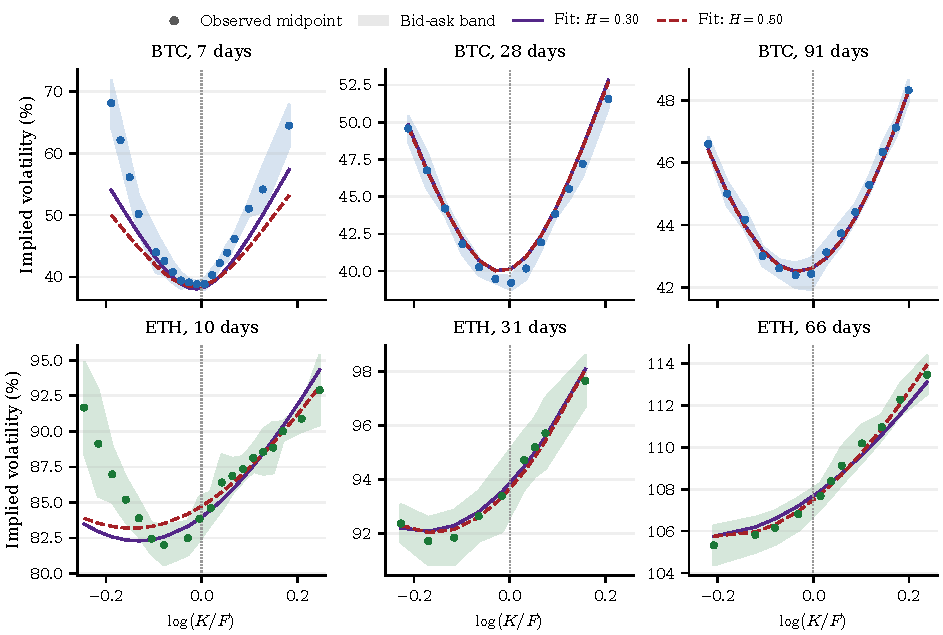
\includegraphics[width=\textwidth]{F1_positive_skew_btc_eth_2026-11-18.pdf}
\caption{Observed Bitcoin and Ether implied-volatility smiles, with bid--ask bands and model fits for both assets at $H=0.30$ (purple, solid) and $H=0.50$ (red, dashed). Bitcoin is observed on 30 June 2023 at 08:00 UTC with maturities 7, 28 and 91 days, and Ether on 26 October 2021 at 08:00 UTC with maturities 10, 31 and 66 days. The 84 retained out-of-the-money Deribit quotes use one common forward per expiry and unchanged coin premiums inverted through $p=\mathrm{Black}(F,K,T,\mathrm{IV})/F$ with unit discounting. Filters require $|\log(K/F)|\le0.25$, forward dispersion at most $0.2\%$, relative premium spread at most $75\%$, implied-volatility spread at most 10 percentage points, positive open interest and archived age proxy at most one hour. For each asset and fixed $H$, one six-parameter calibration covers all three maturities, after pricing qualification at its fitted parameters. Lines connect model values at quoted strikes. The cases were selected retrospectively. All four fits have positive risk-neutral correlation and satisfy $\kappa_2\ge\beta$. They do not identify physical correlation. The $H=0.20$ fit remains withheld pending numerical qualification. Data: Deribit quotes archived on 25 October 2026.}\label{fig:motivation}
\end{figure}

\begin{figure}
\centering
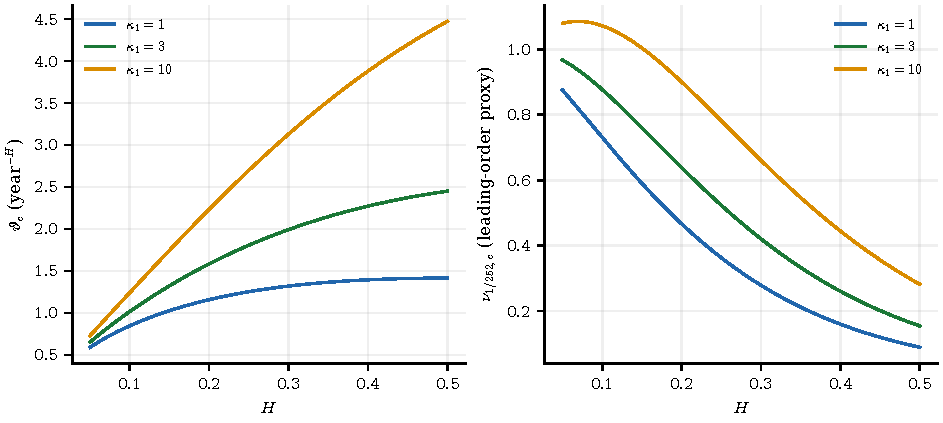
\includegraphics[width=\textwidth]{F2_stability_threshold.pdf}
\caption{The boundary $\gamma=1$ of Proposition~\ref{prop:stationarity}: critical volatility-of-volatility $\vartheta_c$ in year$^{-H}$ (left) and the leading-order one-day innovation proxy $\nu_{1/252,c}$ (right), for $\kappa_1\in\{1,3,10\}$ year$^{-(H+1/2)}$. The closed form \eqref{eq:gamma} agrees with independent spectral quadrature at $H\in\{0.1,0.3,0.5\}$ to a maximum relative difference $1.8\times10^{-12}$.}\label{fig:threshold}
\end{figure}

\begin{figure}
\centering
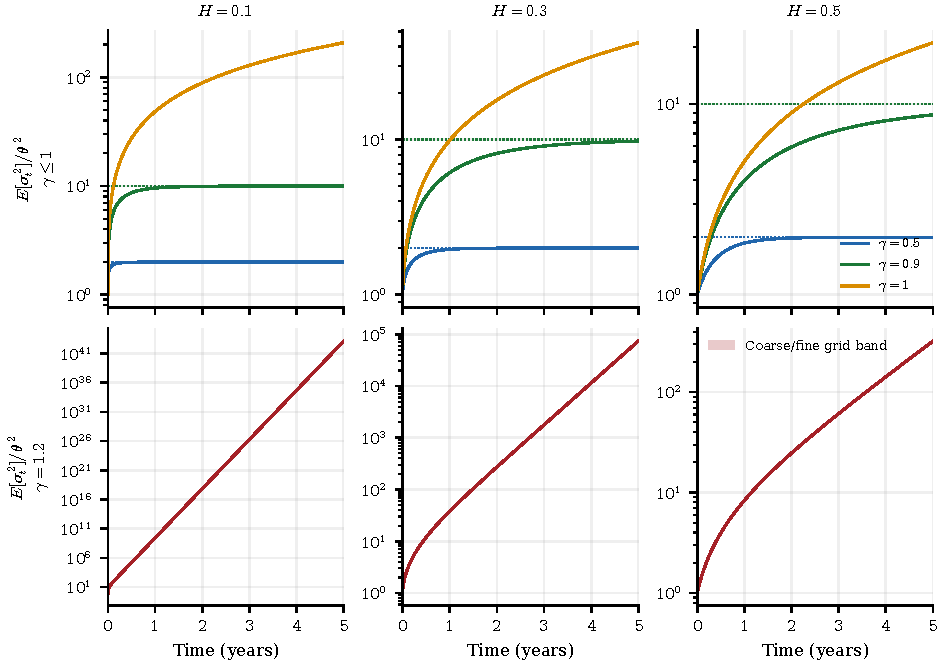
\includegraphics[width=\textwidth]{F3_second_moment_curves.pdf}
\caption{Linear-drift second moments $\E[\sigma_t^2]/\theta^2$ for $\sigma_0=\theta$, $\kappa_1=2$, $\kappa_2=0$ and $H\in\{0.1,0.3,0.5\}$. The top row has $\gamma\in\{0.5,0.9,1\}$, with limits $1/(1-\gamma)$ marked when $\gamma<1$. The bottom row shows $\gamma=1.2$ on separate logarithmic axes. Finite-horizon moments remain finite for every $\gamma$, and the threshold concerns divergence as $t\to\infty$. The kernel-weighted piecewise-linear product-integration solve uses 4,000 and 8,000 steps per year, with shading spanning the two solutions. The largest relative refinement difference is $1.94\%$, at the fractional startup, and it falls below $0.211\%$ after one trading day. The largest terminal difference is $0.0614\%$. Classical-kernel curves agree with the exact solution of the ordinary differential equation within $2.0\times10^{-8}$ relative error. These differences are refinement diagnostics and not rigorous error bounds.}\label{fig:moments}
\end{figure}

\begin{figure}
\centering
% One file for both panels, written by ../replication/rough_logsv_w3_figure.py from F4_quadratic_drift.json and F4_right_panel_time_averaged.json.
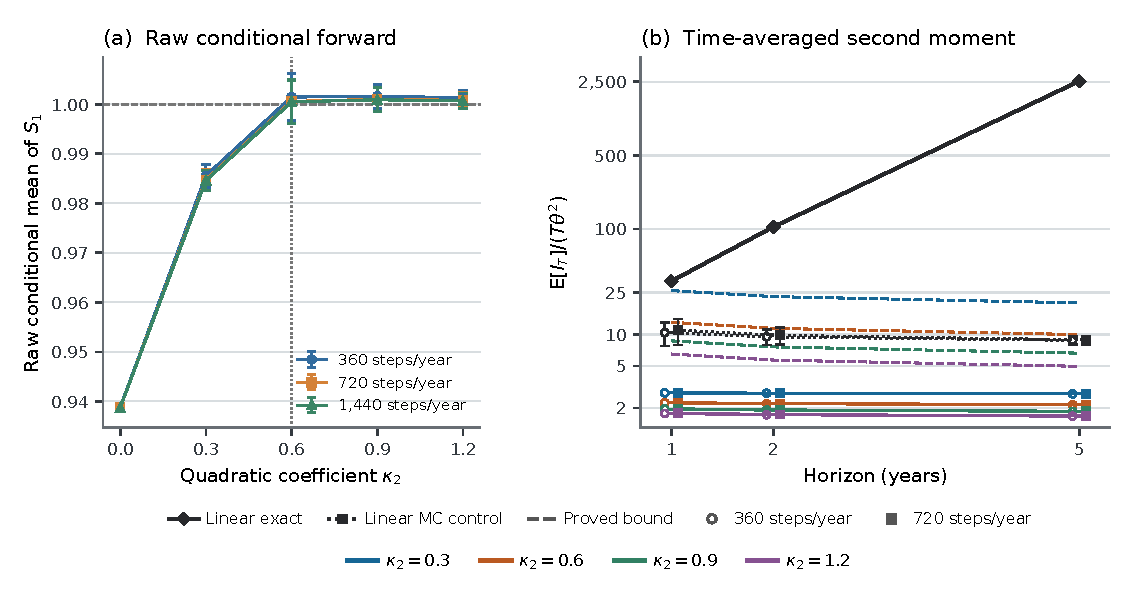
\includegraphics[width=\textwidth]{F4_time_averaged.pdf}
\caption{Quadratic-drift diagnostics for the three-factor kernel at $H=0.1$. Panel (a) shows the raw conditional price means of Table~\ref{tab:martingale} with one per-path standard error. The lines mark a unit forward and $\kappa_2=\beta$. Panel (b) shows the time-averaged second moment $\E[I_T]/(T\theta^2)$ at $T=1,2,5$ years on a logarithmic scale, for $\sigma_0=\theta=0.4$, $\kappa_1=2$, $\rho=0$ and $\vartheta=1.2$ ($\gamma_N=1.0433$), with the nodes and weights of the one-year kernel at every horizon. Diamonds give the exact linear-drift values $32.04$, $104.88$ and $2{,}540.28$. Dashed lines give the bounds \eqref{eq:cesaro} of Proposition~\ref{prop:cesaro}, which hold for every $\vartheta$. Solid lines give the Monte Carlo estimates for $\kappa_2>0$, and the dotted line gives the Monte Carlo estimates for $\kappa_2=0$ as a control. Open circles and filled squares denote 360 and 720 steps per year, horizontally offset, with one standard error from 40 batch means. Each simulated cell uses 200{,}000 paths and the seed-3 stream of Table~\ref{tab:martingale}.}\label{fig:martingale}
\end{figure}

% [GENERATED 2026-11-17 rewritten after the rerun W3 (../agents/sol_results_rough_logsv_W3_2026-11-17.md). Numbers: ../replication/results/F4_right_panel_time_averaged.json, bounds from ../replication/rough_logsv_growth_rate.py.]
Panel (b) of Figure~\ref{fig:martingale} holds the three nodes and weights fixed from one to five years. At $\vartheta=1.2$ the linear three-factor model is above its critical volatility-of-volatility of $1.1748$. Its exact time-averaged second moment $\E[I_T]/(T\theta^2)$ increases from $32.04$ at one year to $104.88$ at two years and $2{,}540.28$ at five years. A separate one-year comparison shows how the linear threshold depends on the kernel. At $\vartheta=1$ the same three-factor kernel has $\gamma_N=0.72$ and an exact one-year ratio $\E[\sigma_1^2]/\theta^2$ of $3.5789$, while the fractional kernel has $\gamma=1.11$ and a numerical one-year ratio of about $32{,}638$.

With quadratic drift, Proposition~\ref{prop:cesaro} bounds the same time average for every $\vartheta$. At five years the bounds \eqref{eq:cesaro} are $19.87$ for $\kappa_2=0.3$ and $4.97$ for $\kappa_2=1.2$. The exact linear-drift value exceeds these bounds by factors of $128$ and $511$, and the comparison uses no simulation. The Monte Carlo estimates for $\kappa_2>0$ lie below their bounds in all 24 cells. At five years and 360 steps per year the estimates decrease from $2.725$ at $\kappa_2=0.3$ to $1.676$ at $\kappa_2=1.2$. Halving the time step raises the estimates by $0.2\%$ to $0.4\%$, and the largest $0.1\%$ of paths contribute $0.5\%$ to $4.8\%$ of each estimate. All cells had zero fallback and floor events.

The estimates for $\kappa_2=0$ show why the simulation alone would not support a statement about stability. At five years the 360-step sample mean of the time average is $8.77$ against the exact $2{,}540.28$, and the sample mean of $\sigma_5^2/\theta^2$ is $16.07$ against the exact expectation $16{,}366.89$. The largest $0.1\%$ of paths contribute $39\%$ to $62\%$ of the linear-drift time averages, which indicates that the exact moment is carried by paths rarer than a sample of 200{,}000 resolves. A simulated moment that stays flat is therefore not evidence of a bounded moment. For $\kappa_2>0$ the comparison in panel (b) rests on Proposition~\ref{prop:cesaro}, and a uniform pointwise bound remains open.
% [END GENERATED 2026-11-17]

% [END REVISED 2026-10-30]

\clearpage
\section{Conclusions and open problems}\label{sec:conclusion}

% [GENERATED 2026-11-17 conclusions restated for the results R1-R4]
We extended log-normal stochastic volatility with quadratic drift to a fractional Volterra equation and proved that it has a unique global non-negative solution with finite moments (Theorem~\ref{thm:wellposed}). For linear drift, exact conditional moments give expected integrated variance and conditional squared VIX. Uniform second-moment boundedness is equivalent to $\gamma<1$, with limiting value $\theta^2/(1-\gamma)$, and above the threshold the second moment grows at the rate $\lambda^*$ of Proposition~\ref{prop:growth}. The explicit constant in \eqref{eq:gamma} makes the threshold reproducible. With a positive quadratic coefficient, the long-run expected integrated variance per unit time is at most $\theta\max(\theta,\kappa_1/\kappa_2)$ for every $\vartheta$ and every $H$ (Proposition~\ref{prop:cesaro}). For the constant kernel the second moment is uniformly bounded (Proposition~\ref{prop:classical_qd}). Theorem~\ref{thm:martingale} gives the martingale property of the price for $\kappa_2\ge\beta$. The change of measure preserves the quadratic polynomial drift, and its density is a true martingale when $\kappa_2^{\Q}\ge0$. Admissible mean-reverting parameters require the restrictions in Proposition~\ref{prop:closure}.

% [REVISED 2026-11-17 after the rerun W3. Numbers: ../replication/results/F4_right_panel_time_averaged.json and ../replication/rough_logsv_growth_rate.py.]
The linear threshold must be evaluated for the kernel used in a simulation. At $H=0.1$ and $\kappa_1=2$ the three-factor kernel of Figure~\ref{fig:martingale} has critical volatility-of-volatility $1.17$, against $0.95$ for the fractional kernel. Above the three-factor threshold, at $\vartheta=1.2$, the exact time-averaged second moment of the linear-drift model is $2{,}540\,\theta^2$ at five years. Proposition~\ref{prop:cesaro} bounds the same average by $19.9\,\theta^2$ for $\kappa_2=0.3$ and by $5.0\,\theta^2$ for $\kappa_2=1.2$, and the simulated estimates lie below the bounds at all three maturities. A sample of 200{,}000 paths understates the exact linear-drift average by a factor of about $290$, so that a flat simulated moment is not evidence of stability. The marked order-flow construction identifies the candidate drift and covariance, and Proposition~\ref{prop:markov} establishes a stopped constant-kernel limit. The singular-kernel construction is an open problem with additional jump and tightness requirements.

Several analytic questions remain. Strict positivity of the volatility is open for singular kernels (Conjecture~\ref{conj:wellposed}). A pointwise long-horizon second-moment bound and a stationary law under quadratic drift are open for $H<1/2$. The converse martingale statement for $\beta>\kappa_2$ follows from \citet{GuyonJeanninJourdain2026} when $\kappa_2=0$ and the kernel is $K^N$. For $0<\kappa_2<\beta$ and for the fractional kernel it is Conjecture~\ref{conj:supermartingale}. For the order-flow limit, Remark~\ref{conj:limit} explains why limit well-posedness alone is insufficient: vanishing jumps, uniform kernel regularity, boundary control and compact containment also have to be established. The selected Bitcoin and Ether calibrations at fixed $H=0.30$ and $H=1/2$ show that positive implied-volatility skew is compatible with positive risk-neutral correlation and the sufficient martingale condition $\kappa_2\ge\beta$. For Bitcoin, the rough fit reduces the equal-maturity weighted root-mean-square error by 9.4\%, with an improvement that is not uniform across maturities. The $H=0.30$ fit places 27 of 45 prices within their bid--ask bands, compared with 28 for $H=1/2$; the quote-level errors and pricing checks are reported in Section~\ref{sec:illustrations}. For Ether, both fixed-$H$ fits place 33 of 39 prices inside their bands; the rough fit's weighted root-mean-square error is 18.3\% higher within the imposed bounds. The $H=0.20$ calibration remains gated. This focused in-sample illustration does not estimate $H$, establish an out-of-sample preference for roughness or identify physical leverage.
% [END GENERATED 2026-11-17]


% [QF 2026-10-31] unnumbered sections required or offered by the journal style; placeholders for the authors.
\section*{Acknowledgements}
\todo{Acknowledgements, if any.}

\section*{Disclosure statement}
\todo{Confirm the journal's standard wording, e.g. ``No potential conflict of interest was reported by the authors.''}

\section*{Data and code availability}
\todo{Confirm: the implementation is in the open-source package StochVolModels (\url{https://github.com/ArturSepp/StochVolModels}); replication scripts and the sealed Deribit snapshot of 25 October 2026 are in the companion \texttt{replication/} folder.}

\section*{Supplemental material}
\todo{Appendix~\ref{sec:conditional_mc} refers to a supplement (earlier scheme and moment-fitted kernel). Either describe the supplemental file here or remove the reference.}

\bibliographystyle{rQUF}
\bibliography{rough_volterra_lognormal_sv_qf}

\appendices

\section{Proofs}\label{app:proofs}

% [GENERATED 2026-10-08]
\begin{proof}[Proof of Lemma~\ref{lem:factors}] Write $\D Z_s=(\kappa_1+\kappa_2\sigma^N_s)(\theta-\sigma^N_s)\,\D s+\vartheta\sigma^N_s\,\D W^\sigma_s$ and $U^{i}_t=\int_0^te^{-x_i(t-s)}\D Z_s$. Then $\sigma^N_t=\sigma_0+\int_0^tK^N(t-s)\,\D Z_s=\sigma_0+\sum_iw_iU^i_t$, and It\^o's formula gives $\D U^i_t=-x_iU^i_t\,\D t+\D Z_t$. The processes $\sigma^{(i)}=\sigma_{0,i}+U^i$ solve \eqref{eq:factors}, and $\sum_iw_i\sigma^{(i)}=\sigma_0+\sum_iw_iU^i=\sigma^N$. For $s\ge t$, $\int_0^te^{-x_i(s-r)}\D Z_r=e^{-x_i(s-t)}U^i_t$, which gives \eqref{eq:theta_N}.
\end{proof}

% [GENERATED 2026-11-17 proof of global well-posedness with quadratic drift (R1)]
\begin{proof}[Proof of Theorem~\ref{thm:wellposed}] Write $b(x)=c_0+c_1x-dx^2$, and for $n\ge1$ define the truncated drift
\begin{equation*}
b_n(x)=b\big(\min\{\max\{x,-n\},n\}\big).
\end{equation*}
Both kernels satisfy the regularity condition (2.5) of \citet{AbiJaberLarssonPulido2019}. The fractional kernel satisfies it with exponent $2H$ by their Example~2.3(ii), and $K^N$ satisfies it with exponent one because it is bounded and Lipschitz. Both kernels are completely monotone and therefore satisfy their condition (3.4) by their Example~3.7. Constants $C$ below depend on $p$, $T$, $K$ and the coefficients, and they do not depend on $n$.

\emph{Step 1: truncation and non-negativity.} The function $b_n$ is bounded and Lipschitz, and $x\mapsto\vartheta x$ is Lipschitz. Theorem~3.3 of \citet{AbiJaberLarssonPulido2019} gives a unique continuous strong solution $\sigma^n$ of \eqref{eq:sve_general} with $b_n$ in place of the drift $b$. The coefficients are continuous with linear growth, $b_n(0)=c_0\ge0$, and the diffusion coefficient vanishes at zero. Their Theorem~3.6 therefore gives a non-negative continuous weak solution, and pathwise uniqueness identifies its law with the law of $\sigma^n$. Thus $\sigma^n_t\ge0$ for all $t$, almost surely.

\emph{Step 2: one-sided bound.} For $x\ge0$ we have $b_n(x)\le c_0+c_1^+x$, where $c_1^+=\max(c_1,0)$. Since $K\ge0$ and $\sigma^n\ge0$,
\begin{equation}\label{eq:one_sided}
0\le\sigma^n_t\le\sigma_0+c_0\int_0^tK(u)\,\D u+c_1^+\int_0^tK(t-s)\sigma^n_s\,\D s+N^n_t,\qquad N^n_t=\vartheta\int_0^tK(t-s)\sigma^n_s\,\D B_s .
\end{equation}
The quadratic term has dropped out of the upper bound.

\emph{Step 3: moments uniform in $n$.} Fix $p\ge2$ and $T>0$, and let $f_n(t)=\E[(\sigma^n_t)^p]$, which is bounded on $[0,T]$ by Lemma~3.1 of \citet{AbiJaberLarssonPulido2019}. Jensen's inequality gives $\big(\int_0^tK(t-s)\sigma^n_s\,\D s\big)^p\le\big(\int_0^TK(u)\,\D u\big)^{p-1}\int_0^tK(t-s)(\sigma^n_s)^p\,\D s$. For fixed $t$, $N^n_t$ is the terminal value of the martingale $u\mapsto\vartheta\int_0^uK(t-s)\sigma^n_s\,\D B_s$ on $[0,t]$. The Burkholder--Davis--Gundy and Jensen inequalities give $\E|N^n_t|^p\le C\int_0^tK(t-s)^2f_n(s)\,\D s$. Taking the $p$-th power and expectations in \eqref{eq:one_sided} yields
\begin{equation*}
f_n(t)\le C+C\int_0^t\big(K(t-s)+K(t-s)^2\big)f_n(s)\,\D s,\qquad t\le T .
\end{equation*}
Choose $\varrho>0$ with $C\int_0^Te^{-\varrho u}\big(K(u)+K(u)^2\big)\D u\le1/2$, which is possible because $K+K^2$ is integrable on $[0,T]$. Multiplying the inequality by $e^{-\varrho t}$ and taking the supremum over $t\le T$ gives $\sup_{t\le T}e^{-\varrho t}f_n(t)\le2C$, so that $\sup_n\sup_{t\le T}f_n(t)\le2Ce^{\varrho T}$.

\emph{Step 4: supremum bound.} On $x\ge0$, $|b_n(x)|\le c_0+|c_1|x+dx^2$, so Step~3 with $2p$ in place of $p$ bounds $\sup_{t\le T}\E|b_n(\sigma^n_t)|^p$ uniformly in $n$. Lemma~2.4 of \citet{AbiJaberLarssonPulido2019} then gives $\E\big[\sup_{t\le T}(\sigma^n_t)^p\big]\le C$ for $p>\max\{2,1/H\}$, and for $p>2$ in the case of $K^N$. With $\tau_n=\inf\{t\ge0:\sigma^n_t\ge n\}$, Markov's inequality gives
\begin{equation}\label{eq:tau_n}
\P(\tau_n\le T)\le Cn^{-p} .
\end{equation}

\emph{Step 5: local uniqueness and removal of the truncation.} Let $X$ and $Y$ be continuous adapted processes and let $\tau$ be the first time that $|X|$ or $|Y|$ reaches $n$. Assume that, up to $\tau$, both satisfy \eqref{eq:sve_general} with the same Brownian motion and with drifts that coincide with $b$ on $[-n,n]$. On $\{t\le\tau\}$ both drift integrands equal $b$ evaluated in $[-n,n]$, where $b$ is Lipschitz, and the indicator $\one_{\{s\le\tau\}}$ can be inserted in both integrals. The function $\Delta(t)=\E\big[|X_t-Y_t|^2\one_{\{t\le\tau\}}\big]$ therefore satisfies $\Delta(t)\le C_n\int_0^t\big(K(t-s)+K(t-s)^2\big)\Delta(s)\,\D s$, and the argument of Step~3 gives $\Delta\equiv0$, that is, $X=Y$ on $[0,\tau]$. In particular $\sigma^m=\sigma^n$ on $[0,\tau_n]$ for $m\ge n$, the times $\tau_n$ increase, and $\tau_n\to\infty$ almost surely by \eqref{eq:tau_n}. The limit $\sigma=\lim_n\sigma^n$ is continuous and non-negative. The limit solves \eqref{eq:sve_general} on $[0,\infty)$, because $b_n(\sigma^n)=b(\sigma)$ on $[0,\tau_n]$ and stochastic integrals of integrands that agree on an event agree on that event. The same local argument gives pathwise uniqueness among continuous solutions. The moment bound follows from Step~4 and Fatou's lemma, first for large $p$ and then for every $p\ge1$ by Jensen's inequality.
\end{proof}
% [END GENERATED 2026-11-17]

% [REVISED 2026-10-30 a priori moment bound replaces the forward reference to Proposition second]
\begin{proof}[Proof of Proposition~\ref{prop:mean}] For $\kappa_2=0$ the coefficients are globally Lipschitz with linear growth. Lemma~3.1 of \citet{AbiJaberLarssonPulido2019} gives $\sup_{s\le T}\E[\sigma_s^2]<\infty$ on every finite horizon, and their Example~2.3(ii) verifies the kernel regularity. The stochastic integral in \eqref{eq:flow} is square integrable since $K\in L^2_{\rm loc}$, and has zero conditional mean. Therefore $m_t(s)=\Theta^t_s+\kappa_1\int_t^sK(s-r)(\theta-m_t(r))\,\D r$. Writing $\phi=m_t-\theta$ gives $\phi=\psi_t-\kappa_1K*\phi$ on $[t,\infty)$, so \eqref{eq:resolvent} yields $\phi=\psi_t-R*\psi_t$. At $t=0$, $\psi_0\equiv\sigma_0-\theta$, giving the unconditional mean. For the fractional kernel, $\widehat R(z)=\kappa_1/(z^\alpha+\kappa_1)$, which inverts to \eqref{eq:resolvent_frac}. When $\kappa_1=0$, $R=0$.
\end{proof}

\begin{proof}[Proof of Proposition~\ref{prop:second}] Subtracting the equation for $m_t$ from \eqref{eq:flow}, the centred process $\chi_s=\sigma_s-m_t(s)$ solves $\chi=-\kappa_1K*\chi+K*\D M$ on $[t,\infty)$, with $\D M_r=\vartheta\sigma_r\,\D W^\sigma_r$. The process $G*\D M$ solves the same linear equation, because $G=K-\kappa_1K*G$, by \eqref{eq:resolvent} when $\kappa_1>0$ and directly from $G=K$ when $\kappa_1=0$, together with the stochastic Fubini theorem. Uniqueness for the linear equation gives $\chi_s=\int_t^sG(s-r)\vartheta\sigma_r\,\D W^\sigma_r$. It\^o's isometry yields $\E[\chi_s^2\mid\F_t]=\vartheta^2\int_t^sG(s-r)^2v_t(r)\,\D r$, and $v_t(s)=m_t(s)^2+\E[\chi_s^2\mid\F_t]$ because $\E[\chi_s\mid\F_t]=0$. The a priori bound in the proof of Proposition~\ref{prop:mean} makes every term finite.
\end{proof}

\begin{proof}[Proof of Corollary~\ref{cor:ml}] With $\kappa_1=0$, $G=K$ and $m\equiv\sigma_0$. Since $\vartheta^2K(t)^2=a\,t^{2H-1}/\Gamma(2H)$, equation \eqref{eq:cond_second} at $t=0$ reads $v=\sigma_0^2+a\,\mathcal{I}^{2H}v$, where $\mathcal{I}^{2H}$ is the Riemann--Liouville integral of order $2H$. Its solution is $\sigma_0^2E_{2H}(a\,t^{2H})$, and integration term by term gives $\E[I_T]$. The asymptotics follow from $E_{2H}(z)\sim(2H)^{-1}\exp(z^{1/(2H)})$ as $z\to+\infty$ \citep{GorenfloKilbasMainardiRogosin2014}.
\end{proof}

\begin{proof}[Proof of Proposition~\ref{prop:vix}] For continuous paths, $-\tfrac2\Delta\E[\ln(S_{T+\Delta}/S_T)\mid\F_T]=\tfrac1\Delta\E[I_{T+\Delta}-I_T\mid\F_T]=\tfrac1\Delta\int_T^{T+\Delta}v_T(s)\,\D s$. Substituting $v_T=m_T^2+\widetilde R*m_T^2$ from Proposition~\ref{prop:second} and exchanging the order of integration gives \eqref{eq:vix}. Under $K^N$, \eqref{eq:theta_N} makes $\psi_T$ affine in $u$, and \eqref{eq:cond_mean} preserves affinity. The square $m_T^2$ is then a quadratic form in $u$, and so is its integral against $\varpi_T$.
\end{proof}

% [REVISED 2026-11-17 localisation proof completed with Theorem wellposed (R2); proof of the density corollary added]
\begin{proof}[Proof of Theorem~\ref{thm:martingale}]
The stochastic exponential $S/S_0$ is a positive local martingale and hence a supermartingale. By Theorem~\ref{thm:wellposed} the volatility is non-negative and does not explode. For $n>\sigma_0$, define $\tau_n=\inf\{t\ge0:\sigma_t\ge n\}$, with $\inf\varnothing=\infty$. The stopped price is a martingale by Novikov's criterion, because $\int_0^{T\wedge\tau_n}\sigma_s^2\D s\le n^2T$. Define
\begin{equation*}
\left.\frac{\D\widehat\Q^{(n)}}{\D\Q}\right|_{\F_T}=\frac{S_{T\wedge\tau_n}}{S_0}.
\end{equation*}
Then $\widehat W^{(0,n)}_t=W^{(0)}_t-\int_0^{t\wedge\tau_n}\sigma_u\D u$ and $W^{(1)}$ form a two-dimensional Brownian motion under $\widehat\Q^{(n)}$, and $\widehat B=(\beta\widehat W^{(0,n)}+\varepsilon W^{(1)})/\vartheta$ is a Brownian motion. Up to $\tau_n$, the volatility satisfies \eqref{eq:sve_general} with respect to $\widehat B$, with drift
\begin{equation*}
(\kappa_1+\kappa_2\sigma)(\theta-\sigma)+\beta\sigma^2
=\kappa_1\theta-(\kappa_1-\kappa_2\theta)\sigma-(\kappa_2-\beta)\sigma^2.
\end{equation*}
Let $\widehat\sigma$ be the global solution of \eqref{eq:sve_general} driven by $\widehat B$ with $c_0=\kappa_1\theta$, $c_1=\kappa_2\theta-\kappa_1$ and $d=\kappa_2-\beta\ge0$, which exists by Theorem~\ref{thm:wellposed}. Let $\widehat\tau_n$ be the first time that $\widehat\sigma$ reaches $n$. Step~5 of the proof of Theorem~\ref{thm:wellposed} gives $\sigma=\widehat\sigma$ on $[0,\tau_n\wedge\widehat\tau_n]$, and therefore $\tau_n=\widehat\tau_n$. The law of $\widehat\sigma$ does not depend on $n$, so the moment bound of Theorem~\ref{thm:wellposed} and Markov's inequality give $\widehat\Q^{(n)}(\tau_n\le T)\le Cn^{-p}$ with $C$ independent of $n$. Thus
\begin{equation*}
\frac{\E_{\Q}[S_T\one_{\{\tau_n>T\}}]}{S_0}
=\widehat\Q^{(n)}(\tau_n>T)
\ge1-Cn^{-p}\longrightarrow1.
\end{equation*}
Since $\one_{\{\tau_n>T\}}\uparrow1$ almost surely, monotone convergence yields $\E_{\Q}[S_T]=S_0$. A non-negative supermartingale whose expectation is unchanged over $[0,T]$ is a martingale, proving the claim.
\end{proof}

\begin{proof}[Proof of Corollary~\ref{cor:density}] Denote the stochastic exponential in \eqref{eq:density} by $D$. The process $D$ is a positive $\P$-local martingale, and with $\tau_n$ as in the previous proof the stopped process $D_{\cdot\wedge\tau_n}$ is a martingale by Novikov's criterion. Under the measure with density $D_{T\wedge\tau_n}$, the substitution that proves Proposition~\ref{prop:closure} shows that, up to $\tau_n$, the volatility satisfies \eqref{eq:sve_general} with $c_0=\kappa_1\theta$, $c_1=\kappa_2\theta-\kappa_1$ and $d=\kappa_2^{\Q}$. For $\kappa_2^{\Q}\ge0$ the argument of the previous proof gives $\E_{\P}[D_T\one_{\{\tau_n>T\}}]\ge1-Cn^{-p}$, and therefore $\E_{\P}[D_T]=1$.
\end{proof}
% [END REVISED 2026-11-17]


% [GENERATED 2026-10-24]
\begin{proof}[Proof of Proposition~\ref{prop:stationarity}] The mean $m(t)=\theta+(\sigma_0-\theta)E_\alpha(-\kappa_1t^\alpha)$ lies between $\sigma_0$ and $\theta$, so $m^2$ is bounded above and below by a positive constant, and $m^2\to\theta^2$. The kernel $h=\vartheta^2G^2$ is non-negative and integrable: $G(t)\sim t^{\alpha-1}/\Gamma(\alpha)$ at zero with $\alpha>1/2$, and $G$ decays as $O(t^{-1-\alpha})$ for $\alpha<1$ and exponentially at $\alpha=1$. Its positive resolvent has the locally convergent convolution series $\widetilde R=\sum_{j\ge1}h^{*j}$. Tonelli's theorem gives
\begin{equation*}
\int_0^\infty\widetilde R(s)\,\D s
=\sum_{j\ge1}\Big(\int_0^\infty h(s)\,\D s\Big)^j
=\sum_{j\ge1}\gamma^j.
\end{equation*}
If $\gamma<1$, Proposition~\ref{prop:second} gives $\sup v\le\sup m^2/(1-\gamma)$, and dominated convergence in $\widetilde R*m^2$ gives $v(t)\to\theta^2/(1-\gamma)$. If $\gamma\ge1$, then with $\underline m=\min(\sigma_0,\theta)>0$,
$v(t)\ge\underline m^2(1+\int_0^t\widetilde R(s)\,\D s)\to\infty$.
% [GENERATED 2026-11-17] next sentence
This direction needs only $\theta\ne0$. If $m(s)^2\ge\theta^2/4$ for $s\ge s_0$, then $v(t)\ge(\theta^2/4)\int_0^{t-s_0}\widetilde R(s)\,\D s\to\infty$.
For the norm, $\widehat G(z)=1/(z^\alpha+\kappa_1)$ and Parseval's identity imply
\begin{equation*}
\int_0^\infty G^2=\frac1{2\pi}\int_{-\infty}^\infty
\frac{\D\omega}{|\omega|^{2\alpha}+2\kappa_1|\omega|^\alpha\cos(\pi\alpha/2)+\kappa_1^2}.
\end{equation*}
The substitution $\omega=\kappa_1^{1/\alpha}u$ gives the factor $\kappa_1^{1/\alpha-2}$. For $\alpha<1$, substituting $y=u^\alpha$ in the remaining integral and integrating the two complex-conjugate linear factors gives
\begin{equation*}
C(\alpha)=-\frac{\cot(\pi\alpha/2)}{\alpha\sin(\pi/\alpha)}.
\end{equation*}
At $\alpha=1$, direct integration gives $C(1)=1/2$, also the limit of this expression.
\end{proof}

% [GENERATED 2026-11-17 proof of the growth rate (R4)]
\begin{proof}[Proof of Proposition~\ref{prop:growth}] Parseval's identity gives the second expression in \eqref{eq:h_hat}. We apply it to $u\mapsto e^{-\lambda u/2}G(u)$, whose Laplace transform on the imaginary axis is
\begin{equation*}
\widehat G(\lambda/2+\mathrm{i}\omega)=\big((\lambda/2+\mathrm{i}\omega)^\alpha+\kappa_1\big)^{-1}.
\end{equation*}
The function $\widehat h$ is continuous and strictly decreasing, and $\widehat h(0+)=\gamma$ by monotone convergence. For $\kappa_1>0$, dominated convergence gives $\widehat h(\lambda)\to0$ as $\lambda\to\infty$, and for $\kappa_1=0$ the transform is $a\lambda^{-2H}$ with $a$ from \eqref{eq:ml_second}. For $\gamma>1$ the root $\lambda^*$ therefore exists and is unique. Equation \eqref{eq:cond_second} at $t=0$ reads $v=m^2+h*v$. Multiplying by $e^{-\lambda^*t}$ gives the renewal equation $v^*=z+h^**v^*$ for $v^*(t)=e^{-\lambda^*t}v(t)$, with $z(t)=e^{-\lambda^*t}m(t)^2$ and $h^*(t)=e^{-\lambda^*t}h(t)$. The function $h^*$ is a probability density with finite mean $\int_0^\infty u\,h^*(u)\,\D u=|\widehat h'(\lambda^*)|$. The function $z$ is continuous and bounded by a multiple of $e^{-\lambda^*t}$, and is therefore directly Riemann integrable. The key renewal theorem \citep[Chapter~XI]{Feller1971} gives $v^*(t)\to|\widehat h'(\lambda^*)|^{-1}\int_0^\infty z(s)\,\D s$, which is \eqref{eq:growth}. For $\sigma_0=\theta$ we have $m\equiv\theta$ and $\int_0^\infty z(s)\,\D s=\theta^2/\lambda^*$.

For $\gamma=1$ the kernel $h$ itself is a probability density. Its mean $\mu_h$ is finite, because $u\,G(u)^2$ is of order $u^{2\alpha-1}$ at zero and of order $u^{-1-2\alpha}$ at infinity for $\alpha<1$, and decays exponentially at $\alpha=1$. The solution is $v=m^2+\widetilde R*m^2$, where $\widetilde R=\sum_{j\ge1}h^{*j}$ is the renewal density. The renewal theorem gives $t^{-1}\int_0^t\widetilde R(s)\,\D s\to1/\mu_h$. Since $m^2$ is bounded and $m^2\to\theta^2$, splitting the convolution at a fixed distance from $t$ gives $v(t)/t\to\theta^2/\mu_h$.
\end{proof}
% [END GENERATED 2026-11-17]

\begin{proof}[Proof of Proposition~\ref{prop:markov}] For $K\equiv1$, set $\delta=\vartheta/\sqrt n$. The Markov chain $(\sigma^n,P^n)$ has jumps $(\delta\zeta,n^{-1/2}\eta)$ at rate $n\sigma^2$, where $\zeta$ and $\eta$ denote the marks of a trade. For $f\in C_c^\infty((0,\infty)\times\mathbb R)$ its generator is $A_nf(\sigma,p)=n\sigma^2\,\E\big[f(\sigma+\delta\zeta,p+n^{-1/2}\eta)-f(\sigma,p)\big]$. Taylor expansion and the mark moments in \eqref{eq:bias} give
\begin{equation*}
A_nf=\sqrt n\,\vartheta\sigma^2\beta_n\,\partial_\sigma f+\tfrac12\vartheta^2\sigma^2\,\partial_{\sigma\sigma}f+\tfrac12\sigma^2\,\partial_{pp}f+\rho(1-|\beta_n|)\vartheta\sigma^2\,\partial_{\sigma p}f+O(n^{-1/2}),
\end{equation*}
uniformly on compact subsets of $(0,\infty)\times\mathbb R$. Fix the domain $D$ of the proposition. On a neighbourhood of its closure the clip is inactive for all sufficiently large $n$, so the first coefficient equals $(\kappa_1+\kappa_2\sigma)(\theta-\sigma)$ and $|\beta_n|\to0$ uniformly. Thus $A_n$ converges there to the generator of \eqref{eq:markov_limit}. The stopped drift and predictable quadratic-variation rates are uniformly bounded, and the jump sizes tend to zero. These bounds give tightness of the stopped martingale problems, and every limit has continuous paths. The limiting coefficients are locally Lipschitz. On $\overline D$ the covariance matrix is uniformly positive definite because $\sigma\ge\sigma_->0$ and $1-\rho^2=\varepsilon^2/\vartheta^2>0$. Therefore the stopped diffusion law is unique, and the boundary of the rectangle is regular for exit. Localisation of the diffusion-approximation argument of \citet{EthierKurtz1986} identifies the limit as the diffusion stopped on leaving $D$, and the chain's exit overshoot tends to zero with its jump size. These steps prove the stated stopped convergence. Removing the stops requires uniform exit estimates for the chains as $\sigma_-\downarrow0$ and $\sigma_+,R\uparrow\infty$, which are not supplied here.
\end{proof}

% [REVISED 2026-10-30 proof moved here from the proof of Proposition markov (C7)]
\begin{proof}[Proof of Proposition~\ref{prop:classical_qd}] For $K\equiv1$ the volatility is the diffusion $\D\sigma=b(\sigma)\,\D t+\vartheta\sigma\,\D W^\sigma$ on $(0,\infty)$, where $b(\sigma)=\kappa_1\theta-(\kappa_1-\kappa_2\theta)\sigma-\kappa_2\sigma^2$. Its speed density is proportional to
\begin{equation*}
\sigma^{-2}\exp\left(\int \frac{2b(\sigma)}{\vartheta^2\sigma^2}\,\D\sigma\right),
\end{equation*}
which gives \eqref{eq:stationary_density}. Put $A=2\kappa_1\theta/\vartheta^2>0$, $B=2\kappa_2/\vartheta^2>0$ and $c=2(\kappa_1-\kappa_2\theta)/\vartheta^2$. The scale and speed densities are proportional to $\sigma^c e^{A/\sigma+B\sigma}$ and $\sigma^{-c-2}e^{-A/\sigma-B\sigma}$. The scale integrals diverge at both endpoints, excluding access from the interior, while the entrance integrals are finite, so both endpoints are entrance boundaries. The finite speed measure normalises to the stationary law. The factors $e^{-B\sigma}$ and $e^{-A/\sigma}$ make all positive and negative stationary moments finite.
For a deterministic initial state, the generator satisfies
\begin{equation*}
\mathcal L\sigma^2=2\kappa_1\theta\sigma+
(-2\kappa_1+2\kappa_2\theta+\vartheta^2)\sigma^2-2\kappa_2\sigma^3
\le C-c_2\sigma^2
\end{equation*}
for some $C,c_2>0$. The stopped It\^o estimate and localisation therefore give
$\E[\sigma_t^2]\le e^{-c_2t}\sigma_0^2+C(1-e^{-c_2t})/c_2$, proving uniform boundedness.
\end{proof}

% [GENERATED 2026-11-17 proof of the time-averaged bound (R3), restated for both kernels in the amendment of r2]
\begin{proof}[Proof of Proposition~\ref{prop:cesaro}] Let $b(x)=\kappa_1\theta+c_1x-\kappa_2x^2$ with $c_1=\kappa_2\theta-\kappa_1$, and define the semimartingale $Z_t=\int_0^tb(\sigma_s)\,\D s+\vartheta\int_0^t\sigma_s\,\D W^\sigma_s$, so that $\sigma-\sigma_0=K*\D Z$. Both kernels are completely monotone. By Example~3.7 of \citet{AbiJaberLarssonPulido2019} they satisfy their condition (3.4), which includes a non-negative resolvent of the first kind $L$. For the fractional kernel with $\alpha<1$, $L(\D s)=s^{-\alpha}\,\D s/\Gamma(1-\alpha)$ and $L([0,T])=T^{1-\alpha}/\Gamma(2-\alpha)$. At $\alpha=1$, $L=\delta_0$ and $L([0,T])=1$, which is the same expression. Their Lemma~2.6 gives $Z=L*(\sigma-\sigma_0)$. Since $\sigma\ge0$ by Theorem~\ref{thm:wellposed} and $L\ge0$,
\begin{equation}\label{eq:Z_lower}
Z_T=\int_{[0,T]}(\sigma_{T-s}-\sigma_0)\,L(\D s)\ge-\sigma_0\,L([0,T]) .
\end{equation}
The moments of Theorem~\ref{thm:wellposed} make the stochastic integral in $Z$ a martingale. With $m(t)=\E[\sigma_t]$ and $v(t)=\E[\sigma_t^2]$, taking expectations in \eqref{eq:Z_lower} gives
\begin{equation*}
\kappa_2\int_0^Tv(t)\,\D t\le\kappa_1\theta\,T+c_1\int_0^Tm(t)\,\D t+\sigma_0\,L([0,T]) .
\end{equation*}
If $c_1\le0$ we drop the middle term, because $m\ge0$. If $c_1>0$ we use $m\le\sqrt v$ and the Cauchy--Schwarz inequality, $\int_0^Tm(t)\,\D t\le\big(T\int_0^Tv(t)\,\D t\big)^{1/2}=T\sqrt{A_T}$. Division by $T$ gives \eqref{eq:cesaro}, which is a quadratic inequality in $\sqrt{A_T}$. Thus $\sqrt{A_T}$ is at most the positive root $y_T$ of $\kappa_2y^2-c_1^+y-\kappa_1\theta-\sigma_0L([0,T])/T=0$, and $y_T$ increases with the last term.

For the fractional kernel the last term tends to zero as $T\to\infty$. If $c_1\le0$, then $y_T^2\to\kappa_1\theta/\kappa_2$, and $\kappa_1/\kappa_2\ge\theta$ in this case. If $c_1>0$, then $y_T\to\big(c_1+\sqrt{c_1^2+4\kappa_2\kappa_1\theta}\big)/(2\kappa_2)=\theta$, because $c_1^2+4\kappa_2\kappa_1\theta=(\kappa_2\theta+\kappa_1)^2$, and $\theta>\kappa_1/\kappa_2$ in this case. Both cases give \eqref{eq:cesaro_limit}.

For $K^N$ put $k(t)=\int_0^tK^N(s)\,\D s$. We integrate $K^N*L\equiv1$ over $[0,T]$ and exchange the order of integration, which gives $T=\int_{[0,T]}k(T-s)\,L(\D s)$ for every $T>0$. The function $k$ is non-decreasing and $L\ge0$, so that $T\le k(T)\,L([0,T])$. The same identity at $T+a$ gives $T+a\ge k(a)\,L([0,T])$ for every $a>0$, because $k(T+a-s)\ge k(a)$ for $s\le T$. Thus
\begin{equation*}
\frac{1}{k(T)}\le\frac{L([0,T])}{T}\le\frac{1+a/T}{k(a)} .
\end{equation*}
We let $T\to\infty$ and then $a\to\infty$ and obtain $L([0,T])/T\to1/k(\infty)=\ell_N$. The limit of $y_T^2$ is the right-hand side of \eqref{eq:cesaro_limit_N}.
\end{proof}
% [END GENERATED 2026-11-17]

\section{Simulation scheme and validation}\label{app:simulation}

% [CARRIED rough_lognormal_simulation.tex Sec. 2, corrected and aligned with split_simulation.py; moved to the appendix on 2026-10-24]
\subsection{Split-step scheme}\label{sec:split_step}

We approximate the factor system \eqref{eq:factors} on a uniform grid with step $h$ by a symmetric drift--diffusion splitting. In this appendix grid-time state symbols denote the numerical approximation, rather than the exact solution,
\begin{equation}\label{eq:strang}
\boldsymbol\sigma_{t+h}=\mathcal{D}_{h/2}\circ\mathcal{S}_h\circ\mathcal{D}_{h/2}\big(\boldsymbol\sigma_t\big),\qquad \boldsymbol\sigma_t=\big(\sigma^{(1)}_t,\dots,\sigma^{(N)}_t\big),
\end{equation}
following \citet{BayerBreneis2024}, who apply the same splitting to rough Heston. The drift map $\mathcal{D}_\tau$ solves the system of ordinary differential equations
\begin{equation}\label{eq:drift_ode}
\frac{\D\xi^{(i)}}{\D t}=-x_i\big(\xi^{(i)}-\sigma_{0,i}\big)+(\kappa_1+\kappa_2\xi^N)(\theta-\xi^N),\qquad \xi^N=\sum_{i=1}^Nw_i\xi^{(i)},
\end{equation}
over a time $\tau$. The implementation approximates this flow by one classical fourth-order Runge--Kutta step, retaining the quadratic drift and checking every intermediate stage.\footnote{The active helper is \texttt{\_drift\_rk4\_checked}. The frozen-coefficient system has the formal solution $\boldsymbol\xi_\tau=e^{A\tau}\boldsymbol\xi_0+\int_0^\tau e^{Au}b\,\D u$, with $A=-(\kappa_1+\kappa_2\xi^N_0)\one w^\top-\mathrm{diag}(x)$ and $b=(\kappa_1+\kappa_2\xi^N_0)\theta\one+\mathrm{diag}(x)\boldsymbol\sigma_0$. The legacy helper \texttt{drift\_ode\_solve3} evaluates the integral as $A^{-1}(e^{A\tau}-I)b$ and requires non-singular $A$, whereas the integral expression also covers singular $A$. Freezing the coefficient omits the change in quadratic damping within the step.} The Jacobian of the full drift is
\begin{equation*}
J(\boldsymbol\xi)=-\mathrm{diag}(x)+\big(\kappa_2\theta-\kappa_1-2\kappa_2\xi^N\big)\one w^\top.
\end{equation*}
The diagnostic $x_N\tau<2.8$ checks the scalar stability interval of the Runge--Kutta step only for the diagonal kernel-decay term. The diagnostic does not control the coupled or nonlinear drift. A frozen-Jacobian check must also examine the eigenvalues of $\tau J$ in the stability region of the Runge--Kutta step, and is itself only local. For example, $N=1$, $x_1=0$, $w_1=1$, $\kappa_1=1000$, $\kappa_2=0$ and $\tau=0.01$ satisfy the diagonal diagnostic, but the amplification of the linear mode is $R_4(-10)=291$, where $R_4(z)=\sum_{k=0}^{4}z^k/k!$ is the stability function of the step. We therefore report step refinement and fallback counts rather than infer global stability or a convergence order from the splitting composition.

The diffusion map $\mathcal{S}_h$ solves $\D\eta^{(i)}=\vartheta\eta^N\D W^\sigma$ for all $i$, with $\eta^N=\sum_iw_i\eta^{(i)}$. Every factor receives the same increment. The weighted sum is a geometric Brownian motion with volatility $\bar w\vartheta$, so the exact solution is
\begin{equation}\label{eq:diffusion_step}
\eta^N_{t+h}=\eta^N_t\exp\Big(-\tfrac12\bar w^2\vartheta^2h+\bar w\vartheta\sqrt h\,Z^\sigma\Big),\qquad \eta^{(i)}_{t+h}=\eta^{(i)}_t+\bar w^{-1}\big(\eta^N_{t+h}-\eta^N_t\big),
\end{equation}
with $Z^\sigma$ standard normal. The diffusion step preserves the sign of $\eta^N$. The Runge--Kutta drift step does not preserve the positivity of $\xi^N$ when $N>1$, because the terms $x_i\xi^{(i)}$ depend on the individual factors.

% [GENERATED 2026-10-09; REVISED 2026-10-30 release history removed]
If a Runge--Kutta stage or a resulting factor, weighted sum, stochastic integral or variance is invalid, the implementation repeats the whole step on that path with the same Gaussian draws and the drift map
\begin{equation}\label{eq:drift_ei}
\xi^{(i)}_\tau=\sigma_{0,i}+e^{-x_i\tau}\big(\xi^{(i)}_0-\sigma_{0,i}\big)+\tau\,\phi_i\,c(s),\qquad \phi_i=\frac{1-e^{-x_i\tau}}{x_i\tau},\qquad c(s)=(\kappa_1+\kappa_2s)(\theta-s),
\end{equation}
in place of the Runge--Kutta step. We use the continuous extension $\phi_i=1$ at $x_i\tau=0$. The end value $s=\sum_iw_i\xi^{(i)}_\tau$ solves $s=A+B\,c(s)$ with $A=\sum_iw_i\big(\sigma_{0,i}+e^{-x_i\tau}(\xi^{(i)}_0-\sigma_{0,i})\big)$ and $B=\tau\sum_iw_i\phi_i$, and we take its positive root. The map integrates the linear decay of the factors exactly and the common drift implicitly. For $\kappa_2\ge0$ the positive root exists whenever $A+B\kappa_1\theta>0$, which holds when the factors are non-negative. The map is first order in $\tau$, so the scheme uses it only as a fallback. A path that still fails receives an artificial whole-step intervention at volatility $10^{-6}$, with its stochastic integral and integrated variance replaced consistently at that level. These interventions are counted and warned about. A reported numerical illustration must have zero such interventions before it is interpreted as evidence about the model.\footnote{Functions \texttt{drift\_ode\_solve\_exp\_implicit} and \texttt{simulate\_split\_step}.}

\subsection{Price step}\label{sec:price_step}

% [GENERATED 2026-10-09] replaces the trapezoidal recovery of J carried from rough_lognormal_simulation.tex
The price step needs the stochastic integral $\int_t^{t+h}\sigma^N\D W^\sigma$ over the step. Under the diffusion map $\mathcal{S}_h$ the weighted sum solves $\D\eta^N=\bar w\vartheta\eta^N\D W^\sigma$, so the stochastic integral of that sub-step is exact,
\begin{equation}\label{eq:J}
J_{t,h}=\int\eta^N\,\D W^\sigma=\frac{\eta^N_{\rm after}-\eta^N_{\rm before}}{\bar w\vartheta},
\end{equation}
where $\eta^N_{\rm before}$ and $\eta^N_{\rm after}$ are the weighted sums before and after $\mathcal{S}_h$ in \eqref{eq:strang}. We use $J_{t,h}$ in place of $\int_t^{t+h}\sigma^N\D W^\sigma$. A recovery of the integral from the volatility increment over the whole step by the trapezoidal rule, as in \citet{Andersen2007}, attributes to the noise the discretisation error of the drift step and of the factor decay. In the scheme, all of the noise enters through $\mathcal{S}_h$, and \eqref{eq:J} is the integral of exactly that noise. Conditional on the volatility path, the orthogonal part of the price noise is Gaussian with variance $\int_t^{t+h}(\sigma^N_u)^2\D u\approx\bar V_{t,h}h$, where $\bar V_{t,h}=\tfrac12\big((\sigma^N_t)^2+(\sigma^N_{t+h})^2\big)$. The log-price and the integrated variance then update as
\begin{equation}\label{eq:price_step}
X_{t+h}=X_t-\tfrac12\bar V_{t,h}h+\rho J_{t,h}+\sqrt{1-\rho^2}\sqrt{\bar V_{t,h}h}\,Z^\perp,\qquad I_{t+h}=I_t+\bar V_{t,h}h,
\end{equation}
with $Z^\perp$ standard normal and independent of $Z^\sigma$. Equations \eqref{eq:J} and \eqref{eq:price_step} are the update of \texttt{split\_step\_f64}. Equation~\eqref{eq:J} is an exact diffusion-substep identity, but the full price update need not preserve the martingale mean exactly at finite $h$. The implementation also supports $\vartheta=0$ through the continuous limit $J_{t,h}=\eta^N_{\rm before}\sqrt h Z^\sigma$, although the model assumptions here have $\varepsilon>0$.

\subsection{Conditional Monte Carlo pricing}\label{sec:conditional_mc}

% [GENERATED 2026-10-09]
Conditional on all volatility-driving random variables, the simulated log return $L_T=X_T-X_0$ is Gaussian with mean $\rho J_T-\tfrac12I_T$ and variance $(1-\rho^2)I_T$, where $J_T$ is the sum of the $J_{t,h}$. With $F=S_0$ under our zero-rate convention, a European payoff on the simulated price $S_T^{(h)}=F e^{L_T}$ has the conditional price of Black's formula with forward and total variance
\begin{equation}\label{eq:conditional_forward}
F_T=F\exp\big(\rho J_T-\tfrac12\rho^2I_T\big),\qquad v_T=(1-\rho^2)\,I_T,
\end{equation}
and the pricer averages these conditional prices over the volatility-driving paths \citep{Willard1997,RomanoTouzi1997}. No draws of $Z^\perp$ are needed. Conditioning is exact for the discretised price law. When the payoff has a finite second moment, the conditional estimator has variance no greater than the plain payoff estimator for that same law. The implementation retains the raw path forwards $F_T$ and reports their sample mean. The implementation applies neither multiplicative forward normalisation nor an additive shift of simulated prices. Sample put--call parity therefore holds relative to the sample forward, and forward discrepancies remain visible. Normalisation by a random sample mean would change the estimator and could conceal discretisation error or a martingale defect.\footnote{Function \texttt{compute\_conditional\_mc\_payoff}, the default of \texttt{rough\_logsv\_mc\_chain\_pricer\_fixed\_randoms}. Inverse payoffs $(S_T-K)^+/S_T$ and $(K-S_T)^+/S_T$ have conditional expectations $N(d_2)-Ke^{v_T}N(d_2-\sqrt{v_T})/F_T$ and $Ke^{v_T}N(\sqrt{v_T}-d_2)/F_T-N(-d_2)$, where $d_2=(\log(F_T/K)-v_T/2)/\sqrt{v_T}$. At $v_T=0$ the conditional price is the payoff at $F_T$. These conditional expectations are taken under the measure of the supplied paths. A coin-numeraire price requires the corresponding measure convention.} Experiments with daily steps, 100{,}000 paths, $H\in\{0.1,0.2\}$, $\rho\in\{-0.7,0.3\}$ and maturities of one and six months gave empirical variance ratios between the plain and conditional estimators from 1.7 to 99. The smallest ratios, 1.7 to 1.9, occurred for out-of-the-money puts at $\rho=-0.7$, for which the volatility path carries more than half of the payoff variance. These sample ratios are diagnostics and do not prove finite payoff variance for every parameter set.\footnote{Source: \texttt{rough\_logsv\_exhibits.py}, case \texttt{CONDITIONAL\_MC\_VARIANCE}, with $\sigma_0=0.5$, $\theta=0.4$, $\kappa_1=2$, $\kappa_2=0$, $\vartheta=0.72$ and strikes $0.8$ to $1.2$, with puts below the forward and calls at and above it. All eight runs had zero fallback and floor events.} The same conditioning gives $\E[S_T^{(h)}]=F\,\E[e^{\rho J_T-\rho^2I_T/2}]$. Tables~\ref{tab:validation} and~\ref{tab:martingale} use its raw sample estimate. Conditioning removes the orthogonal simulation noise and leaves the time-discretisation error. The comparison with the earlier code scheme and the moment-fitted kernel remains in the supplement.

\subsection{Validation against the exact moments}\label{sec:validation}

% [REVISED 2026-11-17 r2. Table B1 and both standard errors: ../replication/results/B1_split_scheme_validation.json.]
Table~\ref{tab:validation} compares the split-step scheme with the exact one-year volatility moments of the same three-factor kernel. All three grids use the 200{,}000 paths and nested increments of Table~\ref{tab:martingale}. In row (c), the mean raw conditional forward at 360 steps is $0.9388093$, and the individual path forwards agree with those of Table~\ref{tab:martingale} on all three grids. Theorem~\ref{thm:martingale} gives a unit price target in rows (a) and (b). In row (c), $\beta=0.6>\kappa_2=0$, and Corollary~2.6 of \citet{GuyonJeanninJourdain2026} gives $\E[S_1]<1$ for this kernel (Section~\ref{sec:measure}). The value of $\E[S_1]$ is not known in closed form.

% [GENERATED 2026-11-17 final pass. Paired refinement changes, standardised deviations and the largest-path share: ../replication/results/B1_split_scheme_validation.json.]
For expected integrated variance, the signed differences from the exact value, divided by the standard error of the 40-batch mean, are $+0.17$, $+0.26$ and $+0.30$ in row (b) and $-0.06$, $+0.08$ and $+0.10$ in row (c) as the grid is refined. The terminal moments $\E[\sigma_1]$ and $\E[\sigma_1^2]$ lie within $1.6$ such standard errors of their exact values in every cell, and the raw conditional forwards of rows (a) and (b) lie within $1.3$ standard errors of the unit target. The three grids share their paths, so the change of an estimate under refinement is measured more precisely than its level. In row (b) the estimate of $\E[I_1]$ rises by $1.0\times10^{-4}$ from 360 to 720 steps and by $0.5\times10^{-4}$ from 720 to 1440 steps, against a batch standard error of the level of $1.1\times10^{-3}$. In row (c) the two changes are $0.0062$ and $0.0008$, with paired batch standard errors $0.0050$ and $0.0018$. The agreement in row (c) is a weak test of the level. The finest-grid estimate is $0.63928$ with batch standard error $0.04668$, which is $7.4\%$ of the exact value $0.63467$, and a single path contributes $5.6\%$ of the estimate. All nine cells had zero fallback and floor events.
% [END GENERATED 2026-11-17]

\begin{table}
\tbl{Split-step estimates at one year for the three-factor kernel with $\sigma_0=0.5$, $\theta=0.4$, $\kappa_1=2$ and $\kappa_2=0$. Rows (a) and (b) use $(\beta,\varepsilon)=(-0.4,0.6)$ and row (c) uses $(0.6,0.8)$. Each grid uses the same 200{,}000 paths with nested increments. Parentheses give the per-path and 40-batch standard errors, respectively. The price column uses the raw conditional forward with $S_0=1$. Exact volatility moments and the unit price targets in (a) and (b) refer to continuous time for the same kernel. In (c) the price is a strict local martingale, and no closed form of $\E[S_1]$ is available.}{%
\begin{tabular}{llrrrr}\toprule
Case & Steps/year & $\E[\sigma_1]$ & $\E[\sigma_1^2]$ & $\E[I_1]$ & $\E[S_1]$ \\
\midrule
(a) $H=0.3$ & 360 & 0.41952 & 0.21367 & 0.23004 & 0.99954 \\
 &  & {\scriptsize (0.00043, 0.00038)} & {\scriptsize (0.00061, 0.00054)} & {\scriptsize (0.00032, 0.00033)} & {\scriptsize (0.00054, 0.00049)} \\
 & 720 & 0.41951 & 0.21366 & 0.23004 & 0.99954 \\
 &  & {\scriptsize (0.00043, 0.00038)} & {\scriptsize (0.00061, 0.00054)} & {\scriptsize (0.00032, 0.00033)} & {\scriptsize (0.00054, 0.00049)} \\
 & 1440 & 0.41952 & 0.21367 & 0.23004 & 0.99954 \\
 &  & {\scriptsize (0.00043, 0.00038)} & {\scriptsize (0.00061, 0.00054)} & {\scriptsize (0.00032, 0.00033)} & {\scriptsize (0.00054, 0.00049)} \\
 & Exact & 0.41906 & 0.21291 & 0.23016 & 1 \\
\midrule
(b) $H=0.1$ & 360 & 0.42475 & 0.29049 & 0.30263 & 0.99939 \\
 &  & {\scriptsize (0.00074, 0.00067)} & {\scriptsize (0.00282, 0.00252)} & {\scriptsize (0.00114, 0.00107)} & {\scriptsize (0.00058, 0.00055)} \\
 & 720 & 0.42469 & 0.29041 & 0.30273 & 0.99934 \\
 &  & {\scriptsize (0.00074, 0.00068)} & {\scriptsize (0.00284, 0.00254)} & {\scriptsize (0.00117, 0.00110)} & {\scriptsize (0.00058, 0.00055)} \\
 & 1440 & 0.42470 & 0.29054 & 0.30278 & 0.99932 \\
 &  & {\scriptsize (0.00074, 0.00068)} & {\scriptsize (0.00287, 0.00255)} & {\scriptsize (0.00118, 0.00111)} & {\scriptsize (0.00058, 0.00055)} \\
 & Exact & 0.42373 & 0.28784 & 0.30245 & 1 \\
\midrule
(c) $H=0.1$ & 360 & 0.42554 & 0.59378 & 0.63228 & 0.93881 \\
 &  & {\scriptsize (0.00144, 0.00131)} & {\scriptsize (0.04662, 0.04276)} & {\scriptsize (0.04361, 0.04227)} & {\scriptsize (0.00067, 0.00061)} \\
 & 720 & 0.42544 & 0.59554 & 0.63844 & 0.93874 \\
 &  & {\scriptsize (0.00144, 0.00131)} & {\scriptsize (0.04854, 0.04458)} & {\scriptsize (0.04776, 0.04628)} & {\scriptsize (0.00066, 0.00061)} \\
 & 1440 & 0.42549 & 0.59828 & 0.63928 & 0.93874 \\
 &  & {\scriptsize (0.00144, 0.00132)} & {\scriptsize (0.05022, 0.04617)} & {\scriptsize (0.04810, 0.04668)} & {\scriptsize (0.00066, 0.00061)} \\
 & Exact & 0.42373 & 0.64737 & 0.63467 & $<1$ \\
\bottomrule\end{tabular}}
\label{tab:validation}
\end{table}

\section{Microstructural reading}\label{sec:micro}

% [GENERATED 2026-10-24 as Section 4; REVISED 2026-10-30 moved to this appendix and compressed (C7). Cut paragraphs (survival of the linear channel, empirical evidence for the kick assumption, per-trade prediction) remain in the 24 October file. Analysis note: rough-lognormal-sv-microstructure-hawkes-foundation-2026-10-24.md (this folder).]
Rough Heston and rough Bergomi are scaling limits of order-driven markets. In each case the limit is fixed by two choices, the volatility state that an order moves and the rate at which orders arrive. Table~\ref{tab:kicks} lists the choices. \citet{JaissonRosenbaum2016} and \citet{ElEuchFukasawaRosenbaum2018} start from a Hawkes process in which each trade adds a constant to the trade intensity, which is the variance, and they obtain the square-root noise of rough Heston. \citet{HagerHorstWagenhoferXu2026} start from orders at a constant rate, each of which adds an i.i.d.\ centred impact to the log-volatility, and they obtain the Gaussian log-volatility of rough Bergomi. The candidate construction below uses a constant signed input kick at a rate proportional to the square of its state. The construction identifies the local noise and drift coefficients of our model. Positivity and global convergence require additional arguments. The drift enters through the law of the kicks by construction, and we say so where it matters. The compensated counting process has predictable quadratic-variation rate equal to the order rate. Thus a constant input kick at rate $\sigma^2$ has noise magnitude $\vartheta|\sigma|$, which agrees with the multiplicative coefficient $\vartheta\sigma$ on a positive branch. The kernel subsequently propagates each kick through the state.

\begin{table}
\tbl{The state that an order moves and the order rate fix the noise of the limit model.}{%
\begin{tabular}{p{2.4cm}p{2.2cm}p{2.6cm}p{1.8cm}p{2.0cm}p{2.95cm}}
\toprule
Limit model & State moved & Kick & Order rate & Noise of the state & Stability norm \\
\midrule
rough Heston & variance $V$ & constant, one-signed & $\propto V$ & $\sqrt V$ & $\|\varphi\|_{L^1}<1$ \\
rough Bergomi & $\ln\sigma$ & i.i.d., centred & constant & constant & none \\
model \eqref{eq:model} & volatility $\sigma$ & constant, signed, biased & $\propto\sigma^2$ & $\vartheta\sigma$ & linear drift: $\gamma<1$ \\
\bottomrule
\end{tabular}}
\label{tab:kicks}
\end{table}

The sign of the kick decides the drift and the stability condition. A one-signed kick on the variance creates the mean feedback $\varphi*V$ of a Hawkes process, and stability is the $L^1$ condition $\|\varphi\|_1<1$. The nearly unstable regime $\|\varphi\|_1\to1$ generates the Mittag-Leffler kernel and the mean reversion of rough Heston. A signed kick of mean zero creates no mean feedback, and stability is the $L^2$ condition $\|k\|_2^2<1$ of \citet{BlancDonierBouchaud2017}. For linear drift, Proposition~\ref{prop:stationarity} gives the corresponding uniform second-moment condition with $k=\vartheta G$. This condition does not apply to the general quadratic-drift model, for which Propositions~\ref{prop:classical_qd} and~\ref{prop:cesaro} give bounds without a restriction on $\vartheta$. The $L^1$ entry in Table~\ref{tab:kicks} describes the underlying Hawkes feedback kernel. The kernel of a signed-kick model is an input rather than a product of criticality, and we take it from the empirical decay of the quadratic feedback in \citet{BlancDonierBouchaud2017}, as \citet{GatheralJusselinRosenbaum2020} do.

% [AUTHOR PARAGRAPH: economic mechanism]
\todo{Economic mechanism paragraph for the kicks, drafted by the authors without AI assistance per project rule. Suggested anchor: each trade moves the volatility by a fixed number of ticks, upward or downward, trades arrive in proportion to the variance, and the market's calming response is a small fixed bias per trade, which therefore grows with the square of the volatility.}

\subsection{A candidate order-flow model}\label{sec:micro_model}

Let $n$ be the number of trades per unit of annualised variance, so that a trade moves the log-price by one tick of size $n^{-1/2}$. Let $K_n$ be a kernel with $K_n(0)<\infty$ that converges to $K$ in $L^2_{\mathrm{loc}}$, for example the shifted kernel $K_n(t)=(t+1/n)^{H-1/2}/\Gamma(H+1/2)$, which is the kernel of \citet{HagerHorstWagenhoferXu2026} up to normalisation. Trades arrive at the jump times $\tau_k$ of a counting process $N^n$ with intensity $n(\sigma^n_{t-})^2$. Each trade carries a sign $\eta_k\in\{-1,1\}$, which is symmetric, and a volatility mark $\zeta_k\in\{-1,1\}$. The volatility and the martingale part of the log-price are
\begin{equation}\label{eq:micro}
\sigma^n_t=\sigma_0+\frac{\vartheta}{\sqrt n}\sum_{\tau_k\le t}K_n(t-\tau_k)\,\zeta_k,\qquad P^n_t=\frac1{\sqrt n}\sum_{\tau_k\le t}\eta_k .
\end{equation}
The law of the mark depends on the volatility before the trade,
\begin{equation}\label{eq:bias}
\P\big(\zeta_k=\eta_k\mid\F_{\tau_k-},\eta_k\big)=\tfrac12\big(1+\rho(1-|\beta_n|)+\eta_k\beta_n\big),\qquad \beta_n=\mathrm{clip}\bigg(\frac{(\kappa_1+\kappa_2\sigma)(\theta-\sigma)}{\sqrt n\,\vartheta\,\sigma^2}\bigg|_{\sigma=\sigma^n_{\tau_k-}},-1,1\bigg),
\end{equation}
with $\beta_n=0$ defined at $\sigma=0$, where the trade intensity is zero. Then $\E[\zeta_k\mid\F_{\tau_k-}]=\beta_n$ and $\E[\eta_k\zeta_k\mid\F_{\tau_k-}]=\rho(1-|\beta_n|)$. The input kick is $\pm\vartheta/\sqrt n$, while the instantaneous state jump is $\pm\vartheta K_n(0)/\sqrt n$. Away from zero the drift enters through a sign bias of order $n^{-1/2}$ per trade.

Let $b(s)=(\kappa_1+\kappa_2s)(\theta-s)$. The compensated input kicks have predictable quadratic-variation rate $(\vartheta^2/n)n\sigma^2=\vartheta^2\sigma^2$, and their mean rate is $\sqrt n\vartheta\sigma^2\beta_n=b(\sigma)$ wherever clipping is inactive. These two rates are the coefficients entering the kernel convolution in \eqref{eq:model}. In that region the quadratic coefficient contributes the level-independent calming bias $-\kappa_2/(\sqrt n\vartheta)$ per trade, and the other coefficients contribute terms proportional to $1/\sigma$ and $1/\sigma^2$.

For positive $s$, every kick is upward only when $b(s)\ge\sqrt n\vartheta s^2$. If $\kappa_1\theta>0$, this is the interval $0<s\le r_n$, where
\begin{equation*}
r_n=\frac{2\kappa_1\theta}{\kappa_1-\kappa_2\theta+\sqrt{(\kappa_1-\kappa_2\theta)^2+4(\kappa_2+\sqrt n\vartheta)\kappa_1\theta}}.
\end{equation*}
For $K\equiv1$ and $n$ large enough that $r_n>\vartheta/\sqrt n$, the jump chain stays above $\min\{\sigma_0,r_n-\vartheta/\sqrt n\}>0$. This lower bound tends to zero with $n$ and does not prove uniform compact containment away from zero. For the shifted fractional kernel, the state jump is $\vartheta n^{-H}/\Gamma(H+1/2)$, whereas $r_n$ is of order $n^{-1/4}$. When $H<1/4$, a downward jump can exceed the protective interval. Between trades, kernel decay also moves the state. Thus the mark bias does not establish positivity of the fractional construction or prove Conjecture~\ref{conj:wellposed}.

The intensity has the quadratic-feedback form $n(\sigma_0+Z^n)^2$, where $Z^n$ is the kernel-weighted signed input. The state marks and price signs are correlated through $\rho$, and the offset $\sigma_0$ shifts the vertex of the quadratic intensity. These features relate the construction to quadratic Hawkes models \citep{BlancDonierBouchaud2017}, but a fixed positive branch has not been established for singular kernels. With zero initial state and no baseline intensity the process is inactive. A nontrivial comparison with \citet{DandapaniJusselinRosenbaum2021} therefore requires their positive baseline intensity or a different non-zero initial input, as discussed below.

\subsection{The Markov case}\label{sec:micro_markov}

\begin{proposition}[Localised Markov approximation]\label{prop:markov}
Let $K_n\equiv K\equiv1$, $\kappa_1>0$, $\theta>0$, $\kappa_2\ge0$ and $\sigma_0>0$. Fix $0<\sigma_-<\sigma_0<\sigma_+$ and $R>0$, and set $D=(\sigma_-,\sigma_+)\times(-R,R)$. The chain $(\sigma^n,P^n)$, started at $(\sigma_0,0)$ and stopped at its first exit from $D$, converges weakly in $D([0,T];\mathbb R^2)$ to the solution of
\begin{equation}\label{eq:markov_limit}
\D\sigma_t=(\kappa_1+\kappa_2\sigma_t)(\theta-\sigma_t)\,\D t+\vartheta\sigma_t\,\D W^\sigma_t,\qquad \D P_t=\sigma_t\,\D W^{(0)}_t,\qquad \D\langle W^{(0)},W^\sigma\rangle_t=\rho\,\D t,
\end{equation}
stopped at its first exit from $D$. The corresponding asset log-price is $X_t=X_0+P_t-I_t/2$.
\end{proposition}

The proof in Appendix~\ref{app:proofs} identifies the generator and proves the stopped diffusion approximation. The proof does not assert global convergence of the chains. Removing the stops requires uniform estimates on their approach to zero and infinity. The candidate limiting diffusion is the classical model of \citet{SeppRakhmonov2023}, and for $\kappa_2>0$ its stationary law and second-moment bounds are given by Proposition~\ref{prop:classical_qd}. This identification explains the role of the calming bias in the candidate limit without supplying a global microscopic limit theorem.

\subsection{Relation to the quadratic Hawkes limit}\label{sec:micro_relation}

Theorem~2 of \citet{DandapaniJusselinRosenbaum2021}, in the numbering of the arXiv version, gives the scaling limit of the purely quadratic Hawkes process with baseline intensity $\mu>0$, Zumbach kernel $k_T=\sqrt{\gamma/T}\,k(\cdot/T)$, $\|k\|_2=1$ and $\gamma\in(0,1)$, in macroscopic time. The limit is $\D P_t=\sqrt{V_t}\,\D B_t$, $V_t=\mu+Z_t^2$ and $Z_t=\sqrt\gamma\int_0^tk(t-s)\sqrt{V_s}\,\D B_s$. Their example takes $k$ proportional to the Mittag-Leffler density $f^{\alpha,\lambda}(t)=\lambda t^{\alpha-1}E_{\alpha,\alpha}(-\lambda t^\alpha)$, which equals the resolvent $R$ of \eqref{eq:resolvent_frac} with $\kappa_1=\lambda$. With $k=G/\|G\|_2$ the limit reads
\begin{equation}\label{eq:djr_limit}
Z_t=\vartheta\int_0^tG(t-s)\sqrt{\mu+Z_s^2}\,\D B_s,\qquad \vartheta=\frac{\sqrt\gamma}{\|G\|_2},
\end{equation}
so that the same parameter $\gamma=\vartheta^2\|G\|_2^2$ controls its stationary second moment. The resolvent identity gives the exact signed-state equation
\begin{equation*}
Z_t=\int_0^tK(t-s)\big[-\kappa_1Z_s\,\D s+\vartheta\sqrt{\mu+Z_s^2}\,\D B_s\big].
\end{equation*}
Formally replacing $\sqrt{\mu+Z^2}$ by $|Z|$ permits the Brownian rotation $\D\widetilde B=\mathrm{sign}_*(Z)\,\D B$, where $\mathrm{sign}_*(0)=1$, and produces a linear multiplicative-noise equation for the signed process $Z$. The rotation does not give that equation for $|Z|$, because taking absolute values does not commute with the Volterra convolution. The rotation also changes correlation with the price Brownian motion according to the sign of $Z$. With $\mu=0$ and the zero initial input of \eqref{eq:djr_limit}, the homogeneous Lipschitz equation has the zero solution. Thus this comparison is a formal signed-process analogy and not an identification with our positive-volatility parameter family.

If a stationary second moment exists, It\^o isometry gives $\E[Z^2]=\mu\gamma/(1-\gamma)$. A large ratio as $\gamma\uparrow1$ describes average second-moment amplification, but does not justify omitting the floor pathwise, particularly near zero. Our construction instead inserts the drift intercept $\kappa_1\theta$ through the mark law, and its positivity and convergence questions are separate.

\subsection{The scaling limit for singular kernels}\label{sec:micro_limit}

\begin{remark}[Open problem: a fractional order-flow limit]\label{conj:limit}
For \eqref{eq:micro}--\eqref{eq:bias}, local $L^2$ convergence of $K_n$ alone cannot imply a continuous scaling limit. The state jumps have magnitude $\vartheta K_n(0)/\sqrt n$. For example, the completely monotone kernels
\begin{equation*}
K_n(t)=K(t+1/n)+n e^{-n^3t}
\end{equation*}
converge to $K$ in $L^2_{\mathrm{loc}}$, since the added spike has squared $L^2$ norm $1/(2n)$, but $K_n(0)/\sqrt n\sim\sqrt n$. Before the first trade the state equals $\sigma_0$, so that trade occurs before $T$ with probability $1-e^{-n\sigma_0^2T}\to1$ and has a diverging state-jump magnitude. Such a jump rules out convergence in the Skorohod $J_1$ topology to a continuous process, irrespective of well-posedness of the proposed limit.
\end{remark}

A viable limit theorem must at least impose $K_n(0)/\sqrt n\to0$. Such a theorem also needs uniform kernel regularity sufficient for tightness, moment and exit estimates for the nonlinear marked processes, control of clipping near zero, identification of every limit point and uniqueness of the target equation. One possible kernel bound to investigate is, for some $\eta>0$ and each $T$,
\begin{equation*}
\int_0^h K_n(s)^2\,\D s+\int_0^T|K_n(s+h)-K_n(s)|^2\,\D s\le C_T h^{2\eta},
\end{equation*}
uniformly in $n$ and $0<h\le1$. This bound is a candidate regularity requirement and not a sufficient-condition theorem for the full nonlinear construction. The shifted fractional example has vanishing jump scale $n^{-H}$, but the sign-preservation difficulty above remains. We therefore leave global convergence to \eqref{eq:model} open. The limits in \citet{DandapaniJusselinRosenbaum2021}, \citet{HorstXuZhang2024} and \citet{HagerHorstWagenhoferXu2026} use their own state spaces, baseline intensities and regularity assumptions, and none is a special case of an established limit theorem for the present construction.

The local drift calculation nevertheless gives a parameter interpretation. The volatility-of-volatility $\vartheta$ scales the signed input kick. The coefficient $\kappa_2$ contributes a level-independent calming bias per trade, and the quadratic arrival rate turns it into quadratic damping. The intercept $\kappa_1\theta$ gives an upward bias at low activity. Under a change of measure, Proposition~\ref{prop:closure} shifts the quadratic coefficient by $\beta\bar\lambda_0+\varepsilon\bar\lambda_1$, subject to the admissibility restrictions stated there. A bias of order $n^{-1/2}$ does not make the drift unidentifiable from tick data: the relevant limitation is that increasing sampling frequency over a fixed time span does not by itself provide consistent drift estimation, whereas longer observation spans carry drift information. The construction is an interpretation of the coefficients and a localised approximation, and its global fractional limit remains an open problem.

% [END GENERATED 2026-10-24 / REVISED 2026-10-30]

\section{Notation and implementation map}\label{app:notation}

% [GENERATED 2026-10-08]
Table~\ref{tab:notation} maps the symbols of this paper to the implementation in StochVolModels version 2.18.0 and to the replication scripts.

\begin{table}
\tbl{Symbols and code names.}{%
\begin{tabular}{p{2.6cm}p{5.2cm}p{6.2cm}}
\toprule
Symbol & Meaning & Code \\
\midrule
$\sigma_0,\theta$ & initial and mean volatility & \texttt{LogSvParams.sigma0}, \texttt{theta} \\
$\kappa_1,\kappa_2$ & linear and quadratic mean reversion & \texttt{kappa1}, \texttt{kappa2} \\
$\beta$ & volatility beta & \texttt{beta} \\
$\varepsilon$ & residual volatility-of-volatility & \texttt{LogSvParams.volvol}, pricer argument \texttt{orthog\_vol} \\
$\vartheta=\sqrt{\beta^2+\varepsilon^2}$ & total volatility-of-volatility & \texttt{LogSvParams.vartheta}; argument \texttt{vartheta} in \texttt{split\_simulation} \\
$\rho=\beta/\vartheta$ & spot-volatility correlation & \texttt{LogSvParams.rho}; argument \texttt{rho} \\
$H$, $K$ & Hurst exponent, kernel \eqref{eq:kernel} & \texttt{H}, \texttt{rough\_kernel.fractional\_kernel} \\
$x_i,w_i$ & nodes and weights of $K^N$ & \texttt{nodes}, \texttt{weights} \\
$\bar w=K^N(0)$ & kernel value at zero & \texttt{weights.sum()}; cap \texttt{w\_bar\_max} \\
kernel rule & quadrature rule or moment fit & \texttt{KernelRule.EUROPEAN}, \texttt{KernelRule.MOMENT\_FIT} \\
$\sigma_{0,i}=\sigma_0/\bar w$ & factor initial values and targets & \texttt{sigma0\_factors} \\
$\sigma^{(i)}_t$, $\sigma^N_t$ & factors and aggregated volatility & rows of \texttt{vol}, \texttt{weights @ vol} \\
$I_t$ & integrated variance & \texttt{qvar} \\
$Z^\sigma,Z^\perp$ & normals of \eqref{eq:diffusion_step}, \eqref{eq:price_step} & \texttt{Z0}, \texttt{Z1} \\
$\mathcal{D}_\tau$, $\mathcal{S}_h$ & drift and diffusion maps & \texttt{\_drift\_rk4\_checked}; diffusion in \texttt{split\_step\_f64} \\
fallback map & drift map \eqref{eq:drift_ei} & \texttt{drift\_ode\_solve\_exp\_implicit} \\
$J_{t,h}$, $J_T$ & stochastic integral \eqref{eq:J} and its sum & \texttt{jump} in \texttt{split\_step\_f64}, \texttt{SplitStepPaths.jump} \\
$F_T$, $v_T$ & conditional forward and variance \eqref{eq:conditional_forward} & \texttt{compute\_conditional\_mc\_payoff} \\
$\gamma=\vartheta^2\|G\|_2^2$ & stability parameter \eqref{eq:gamma} & \texttt{g2\_norm} in \texttt{rough\_logsv\_stationarity\_check.py} \\
$\widehat h$, $\lambda^*$ & transform \eqref{eq:h_hat} and growth rate \eqref{eq:growth} & \texttt{h\_hat}, \texttt{growth\_rate} in \texttt{rough\_logsv\_growth\_rate.py} \\
$\gamma_N$ & stability parameter of $K^N$, Section~\ref{sec:illustrations} & \texttt{markov\_stability\_parameter} in the same script \\
$\nu_\Delta$ & $\Delta$-horizon innovation volatility-of-volatility, Section~\ref{sec:stability} & case \texttt{DAILY\_INNOVATION\_TABLE} of \texttt{rough\_logsv\_stationarity\_check.py} \\
$n$, $\beta_n$ & trades per unit variance, kick bias \eqref{eq:bias} & interpretation only, no code \\
\bottomrule
\end{tabular}}
\label{tab:notation}
\end{table}

\section{Nearest results}\label{app:nearest}

% [GENERATED 2026-10-08; REVISED 2026-11-17] Prior-art list required before any novelty claim. No novelty claim is made in this draft.
% The prior-art sweep for Theorems wellposed and martingale and for Proposition cesaro was run on 17 November 2026
% (project note rough-lognormal-sv-prior-art-sweep-2026-11-17.md). Its entries are the last five sentences below.
The nearest results and their differences are as follows. \citet{GatheralJusselinRosenbaum2020} take $V=a(Z-b)^2+c$. At $c=0$, the signed state satisfies \eqref{eq:qrh_map} with linear drift and negative mean-reversion level, while its volatility is the absolute value of that state. \citet{DandapaniJusselinRosenbaum2021} derive a quadratic-Hawkes limit with a positive variance floor and a signed trend, and Appendix~\ref{sec:micro_relation} states the exact normalised equation and the limits of the floor-free analogy. \citet{ChudasamaIyer2025} extend their framework to asymmetric buy and sell impacts. \citet{BayerFrizGatheral2016} specify a Gaussian Volterra log-variance with deterministic forward-curve and variance-normalisation terms, and \citet{HagerHorstWagenhoferXu2026} derive rough log-normal volatility from order flow with additive log-volatility impacts. \citet{ElEuchRosenbaum2019} and \citet{AbiJaberLarssonPulido2019} treat affine Volterra variance and Riccati transforms, and \citet{JaissonRosenbaum2016} and \citet{ElEuchFukasawaRosenbaum2018} derive related models from nearly unstable Hawkes processes. \citet{AbiJaberIllandLi2022} use a polynomial of a Gaussian Ornstein--Uhlenbeck process. \citet{GuyonJeanninJourdain2026} give general martingale and strict-local-martingale criteria. Their Lemma~3.1 supplies the localisation and non-explosion reduction relevant here, while the natural quadratic-drift representation fails the growth restriction for a direct application of their Theorem~1(B), as discussed in Section~\ref{sec:measure}. Theorem~\ref{thm:wellposed} supplies the non-explosion step through a one-sided moment bound for the non-negative state. \citet{SeppRakhmonov2023} is the classical $H=1/2$ model.
% [GENERATED 2026-11-17 attribution pass] next five sentences
For well-posedness, \citet{PannierJacquier2019} treat a locally Lipschitz drift with linear growth. For the moments under linear drift, \citet{AbiJaberCuchieroPelizzariPulidoSvalutoFerro2024} give the moment equations of polynomial Volterra processes. \citet{Pages2024} and \citet{GnabeyeuPages2025} bound the second moment of an equation stabilised by a deterministic function of time. For the martingale property, \citet{AbiJaberGassiatSotnikov2025} treat signature volatility, and Corollary~2.6 of \citet{GuyonJeanninJourdain2026} covers our model with $\kappa_2=0$. \citet{CarrWillems2019} obtain the generalised inverse Gaussian steady-state law at $H=1/2$.
% [END GENERATED 2026-11-17]



\end{document}
